\chapter{Signal flow}
\label{chap:flow}

From the previous chapter, we know that the cellular machinery of 
transcriptional and metabolic regulation is under-represented in the strongly 
regulated genes and thus hidden from the time-resolved transcriptome data. 
Consequently, the investigation of strong responders only gives insights into
the periphery of the gene regulatory network and functions directly related
to the cellular phenotype. What is largely missing is a holistic picture of
the signaling pathway activity, namely how the external stimulus is translated
to the protein signaling events that propagate through the protein interaction
network and ultimately lead to the measured gene regulation (\ref{fig:signal_flow}).

In the following, we first introduce several classical methods to infer the
enrichment of pathways from the transcriptome data. We point out the drawback
of their implicit assumptions and propose a two-step approach to identify the
causal signal\footnote{We use \emph{signal} and \emph{information} interchangably.} 
flow from membrane receptors to transcription factors. Finally,
we apply this approach in the study of cell-cell communication in the lung
cancer.

\section{Pathway enrichment analyses}
Since the introduction of the microarray technology, pathway analysis has been 
a heavy focus and first choice for gaining insight into the underlying biology 
of differentially expressed genes. Over the past decade, we have seen at least 
three generations of pathway analyses~\citep{Khatri2012}, here we discuss 
their core features and limitations.

\subsection{Over-representation test}
Over-representation test is also called Fisher's exact test, it statistically 
evaluates the fraction of genes in a particular pathway found among the set 
of genes showing significant changes in expression. 
A researcher first chooses genes that are 
differentially over- or under-expressed in a given condition at a certain 
threshold (separate into columns in \ref{table:contigency_table}). Then, for each pathway, the number of genes that are part of the 
pathway is counted. This process is repeated for an appropriate background 
list of genes (e.g., all genes measured on a microarray), 
such that the column sums can be further divided. 
Next, every pathway 
is tested for over- or under-representation based on the frequencies in such 
a $2 \times 2$ contingency table (\ref{table:contigency_table}). 
Fisher has shown that the probability of obtaining any such set of values was 
given by the hypergeometric distribution. To calculate the significance of the
test, i.e. the total probability of observing data as extreme or more extreme 
if the null hypothesis is true, one has to sum up the individual probability
of observing the data and all those of observing more extreme frequencies.

\begin{longtable}{cccc}
\caption[Contingency table example]{
An example of the contingency table used in the pathway enrichment analysis.} \\
\hline
& differentially regulated & not regulated & row sum \\
\rowcolor{Gray} pathway & $a$ & $b$ & $a+b$\\
background & $c$ & $d$ & $c+d$\\
\rowcolor{Gray} column sum & $a+c$ & $b+d$ & $a+b+c+d(=n)$\\
\hline
\label{table:contigency_table}
\end{longtable}

One of the critics on Fisher's exact test is that it only considers a ranked
list of differentially expressed genes and is thus independent of the 
measured fold changes. Second, the generation of the contingency table
requires setting a significance cutoff to count the number of differentially
regulated genes. This procedure introduces a subjective criterion and 
effectively treats the gene regulation as a black-white picture, namely only 
genes above this threshold are considered differentially expressed.
    
\subsection{Gene set analysis}
To avoid the arbitrary significance cutoff and to realize the fact that weaker 
but coordinated changes in sets of functionally related genes (i.e., pathways) 
can also have significant effects, gene set enrichment analysis was suggested~%
\citep{Subramanian2005,Luo2009}. In general,
a pathway-level (gene group level) statistic is calculated from the gene-level 
differential expression between two experimental conditions, and the 
statistical significance is assessed according to the test of
this pathway-level statistic between the pathway (group) of interest and a 
background set.

By considering the coordinated changes in gene expression, gene set analyses 
account for dependence between genes in a certain pathway or group, without
the need to set the artificial cutoff between the differentially and 
non-differentially regulated genes. However,
each pathway is still analyzed independently and thus crosstalks between
pathways are disregarded.

\subsection{Topology-based approach (SPIA)}
Over-representation and gene set analyses only consider the number of genes 
in a pathway to identify significant pathways, and ignore the additional 
information available from various prior knowledge bases. Recently a signaling
pathway impact analysis (SPIA) was proposed~%
\citep{Tarca2009}. SPIA considers the structure and dynamics of an entire 
pathway by incorporating changes in gene expression, types of interactions, 
and the positions of genes in a pathway. 
It calculates the pathway-level statistic from the combinatorial probability 
of perturbation in gene expression and over-representation. 

Not unlike any other approaches based on prior knowledge,
SPIA heavily depends on the true pathway topology, which is highly
context-dependent and remains poorly understood and annotated.

\subsection{NetSearch}
\cite{Steffen2002} further built upon the idea of incorporating 
prior knowledge about the pathway topology and suggested
the inference of signal transduction networks with protein-interaction maps
and expression profiles from DNA microarrays.
It works by first enumerating all possible linear paths
of a specified length through the interaction map starting
at any membrane protein and ending on any DNA-binding
transcription factors.
Microarray expression data are then used
to rank all paths according to the degree of similarity in
the expression profiles of pathway members.
Linear pathways
that have common starting points and endpoints
and of the highest ranks are then combined into the final
model of the branched networks.

Based on the gene expression data of pheromone response in the yeast, the 
NetSearch algorithm accurately reconstructs the MAPK cascade, it also identifies a 
network with other proteins necessary to execute the coordinated processes of 
growth polarization and cell cycle arrest, and reflects the complex topology of 
the interaction network in response to pheromone.

\subsection{Drawback}
All the above methods make the implicit assumption that the expression of genes
and their corresponding protein products are correlated, or the signaling 
pathway activity, which is largely determined by the member protein level, 
can be inferred from the transcriptome data. There has been ongoing debate 
about whether the transcriptome regulation correlates with the proteome
in bacterial and mammalian cells~\citep{Taniguchi2010,Ghazalpour2011}. 

More
often than not, the assumption of correlation either does not hold or strongly depends on the context~\citep{Soufi2009}. 
It has also been shown that the mRNA-protein expression correlation increases 
with time~\citep{Fournier2010}.
As one of the protein classes important in disease, 
transcription factors (TF) remain largely decoupled at the 
protein
and mRNA level, which renders them a highly dynamic and efficient switch that 
can fine-tune the gene expression. Indeed, many of the TFs that regulate physiological
    targets are constitutively present, and their activity is determined
    by posttranslational modifications such as phosphorylation%
    ~\citep{Messina2004}.
Therefore, questions arise about the validity of inferring signaling 
pathway activity based solely on the gene expression level.

\section{Two-step integrative approach to causal signal flow}
We propose here a two-step integrative approach to infer the activated protein signaling
pathways from time-resolved microarray data. As a first step, we apply a
gene set enrichemnt analysis to test the
enrichment of transcription factor target genes, which acts as a proxy of
the transcription factor activity \emph{per se}. Second, the upstream 
signal flow from membrane receptors to transcription factors is predicted 
based on the distance between both end nodes in the protein interaction
network.

\subsection{Identification of activated transcription factors}
We performed gene set enrichment tests, 
using a modified implementation~\citep{Luo2009}.
To this end, we retrieved sets of genes regulated by 
a common transcription factor from MSigDB v3.0 (The Molecular Signature Database, \cite{Liberzon2011}). 
This database contains two major data sources. The first one is mammalian 
transcriptional regulatory motifs from the v7.4 public version of TRANSFAC 
database~\citep{Matys2003b}. Every such motif gene set consists of human 
genes whose promoters (defined as regions -2kb to +2kb around transcription 
start site) contain at least one instance of the motif.
The second data source for transcription factor targets in MSigDB is derived 
from upstream motifs highly conserved among five mammalian species~%
\citep{Xie2005e}. Each motif gene set consists of all human genes whose 
promoters contained at least one conserved instance of the motif.

Individual genes were first ranked according to their response strengths as derived from the 
multidimensional scaling of the normalized time series 
(\ref{sec:response_strength}). The difference in the response strength of both
the transcription factor target gene set and  
the whole transcriptome as a background is tested by a Kolmogorov-Smirnov statistic. 
The transcription factors of the respective significantly differentially regulated
gene sets are deemed active.

\subsection{Signal flow from membrane receptors}
The second step involves inferring how extracellular signal flows from the 
membrane receptors to 
the transcription factors and subsequently induces gene regulation. 
To this end, we assume that the signal flows along the edges of a network 
in a most efficient manner. Consequently, it is 
crucial to be able to measure the proximity between a given pair of receptor and
transcription factor in the protein-protein interaction network. Here we 
compare two distance metrics, one is the shortest path length, and the other
being the mean first passage time based on the idea of random walk.

\subsubsection{Shortest path length}
If one assumes that information propagates in the network in a most parsimonious
or efficient way,
shortest path (SP) length between two nodes in the network is a classical way to
assess the distance between these two nodes and thus possible route of signal flow
(\ref{sec:shortest_path}). Several variations of the 
shortest path approach have been used in extracting 
phenotype-associated and previously unknown genes~%
\citep{Zhou2002,Managbanag2008}.

When multiple target genes exist, the well-known graph-theoretical concept of a Steiner tree is often used in place of a set of shortest paths. Given a set of nodes to be connected, a Steiner tree is an acyclic subgraph (a tree) connecting all these nodes while using the minimum number of edges. In a Steiner tree, the individual path from the putative causal gene (the root of the tree) to each of the target genes does not need to be the shortest, but the size (i.e., the number of edges) of the whole tree is minimized. The Steiner tree approach has been used to find new functional associations for proteins~\citep{Huang2009,Bailly-Bechet2011}.

\cite{Vinayagam2011} used several features based on the shortest PPI path 
information from membrane receptors to transcription factors to
predict a directed human protein-protein interaction 
network, which contains edge directions
inferred by a naive Bayesian classifier.
Based on this directed PPI together with time-resolved protein phosphorylation data,
they were able to both reconstruct time-ordered events and
predict novel players in the signal transduction of the activated epidermal growth factor and extracellular signal-regulated kinase (EGF/ERK) signaling cascade.

In this work, we focus on a consolidated PPI network called HIPPIE 
(\textbf{H}uman \textbf{I}ntegrated \textbf{P}rotein-\textbf{P}rotein 
\textbf{I}nteraction r\textbf{E}ference), which has a confidence scoring 
scheme that reflects the amount and quality of evidence for a given PPI. 
We first determined an appropriate cutoff score to prune the network.
Then for each cytokine receptor/transcription factor pair in question,
we calculated the length of the shortest path between the two
using the unweighted breadth-first search algorithm,
as implemented in the R package \texttt{igraph}~\citep{Csardi2006}.
We use these lengths as base metric for the probability 
of signal actually flowing through the pathway.

Intuitively, the shortest path is only the best scenario of all possible routes
of information flow in the network. Therefore, it simply ignores the 
neighborhood or global structure around the shortest path when calculating
distances. Another limitation of the shortest path distance metric has to do
with the small characteristic path lengths in a small-world networks~%
\citep{Watts1998}, such that any nodes can be reached from any other nodes
within only few hops when traveling on the shortest path and the shortest path
metric loses its discriminative power. Since most biological
and real-world networks demonstrate the small-world feature~%
\citep{Barabasi2004}, this limitation
has to be kept in mind when working with the shortest path.

\subsubsection{Mean first passage time}
Another category of distance metric in networks is the 
so-called flow-based methods, which compute the fraction of flow going through each intermediate node/edge. In the case of current flow approach, the network is modeled to mimic the behavior of current in an electronic circuit, where each edge has an associated resistance~\citep{Missiuro2009}. The current flow approach is
also shown to be equivalent to a random walk in the network~%
\citep{Doyle2000}.

The mean first passage time (MFPT) is defined as the average time/steps 
necessary for 
a random walker starting from a source node to reach a target node for the
first time. It has been shown that MFPT can be used to detect community
structures in the protein interaction network of yeast~\citep{Zhou2003}. 
Recently, a random walk with restart approach was applied to associate
target gene sets to reference datasets as an alternative to 
over-representation-based enrichement analyses~\citep{Glaab2012}. 
Further examples include a random walk-based software tool for functional
analyses of cellular networks with genomic data integrated~\citep{Komurov2012a}.
Moreover,
the usefulness of MFPT became evident by the fact that the pairwise MFPT 
matrix is sufficient to reconstruct the full network topology~%
\citep{Wittmann2009}.

MFPT can be calculated analytically by solving a linear equation system~%
\citep{Kampen2007}. Consider the special case of a linear chain 
(\ref{fig:mfpt_calculation}) and suppose the random walker starts from node 
$x$ at a certain time $t$, with the probability of jumping to adjacent nodes
being equal, we have
\begin{equation}
\tau(x,y) - 1 = \frac{1}{2}\tau(x-1,y) + \frac{1}{2}\tau(x+1,y)
\label{eq:mfpt}
\end{equation}
where $\tau(x,y)$ denotes the mean first passage time of reaching $y$ and 
starting at $x$, which can be decomposed of 1 time unit needed to reach the
next time step $t+1$ and the travel time to the target node $y$ at $t+1$.
Since the random walker can be at either node $x-1$ or $x+1$ at $t+1$, each
with equal probability, we express the mean first passage time to $y$ at
time step $t+1$ as the right-hand-side of \ref{eq:mfpt}.

\begin{figure}[!ht]
\begin{center}
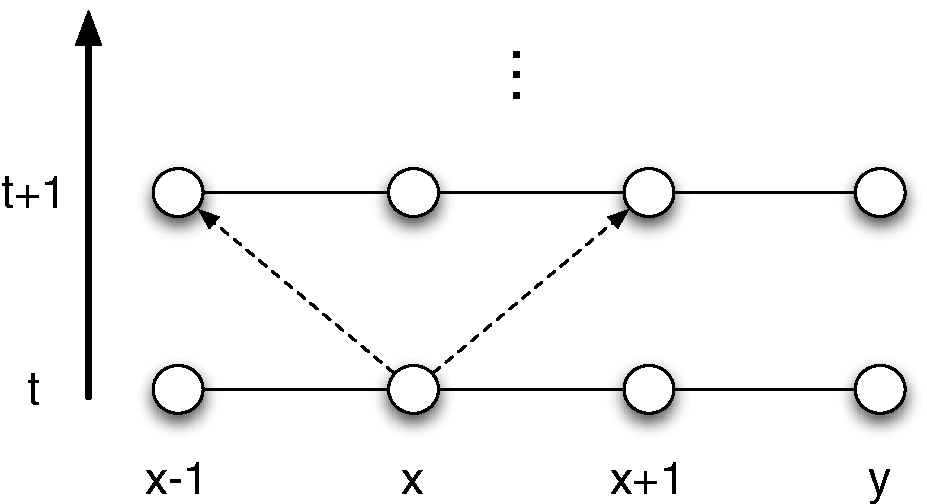
\includegraphics[width=0.8\textwidth]{mfpt_calculation.pdf}
\end{center}
\caption[MFPT calculation]{
{\bf The calculation of MFPT on a linear chain.}
The same linear chain consisting of 4 nodes is depicted in different time 
slices ($t,t+1,\ldots$), 
a random walker starting from node $x$ at time $t$ can jump to either $x-1$ 
or $x+1$ at time $t+1$.
}
\label{fig:mfpt_calculation}
\end{figure}

\ref{eq:mfpt} can be rewritten and generalized to an arbitrary graph, i.e.
the mean first passage time from all possible nodes to a target node $y$
can be expressed as a linear equation system
\begin{equation}
(\tilde{\mathbf{L}}-\boldsymbol{\beta}^y) 
\begin{pmatrix}
\tau(1,y)\\
\tau(2,y)\\
\vdots\\
\tau(N,y)
\end{pmatrix}
= \boldsymbol{\delta}
\label{eq:mfpt_system}
\end{equation}
where 
\begin{equation}
\delta_i=
\begin{cases}
0 & i=y\\
1 & \textnormal{otherwise}
\end{cases}
\end{equation}
and $\tilde{\mathbf{L}}$ is the normalized graph Laplacian and
\begin{equation}
\tilde{L}_{ij}=
\begin{cases}
1 & i=j\\
-1/deg(i) & i \neq j \ \textnormal{and}\ i \ \textnormal{is adjacent to}\ j \\
0 & \textnormal{otherwise}
\end{cases}
\end{equation}
where $deg(i)$ is the degree of node $i$. $\boldsymbol{\beta^y}$ 
is the boundary condition
matrix that ensures $\tau(y,y)=0$, more specifically
\begin{equation}
\beta^y_{ij}=
\begin{cases}
\tilde{L}_{ij}-1 & i=j=y\\
\tilde{L}_{ij} & i=y\\
0 & \textnormal{otherwise}
\end{cases}
\end{equation}
It is easy to see that $\tilde{\mathbf{L}}$ can be pre-calculated and then be 
reused to estimate the
MFPT for each target node $y$. Moreover, the calculations
for different targets are independent and hence can be
determined in parallel. As networks in biology are often
sparse, the equation system in \ref{eq:mfpt_system}
is suitably represented by a sparse matrix. The matrix
is positive semi-definite and can be solved by the LGMRES algorithm~%
\citep{Baker2005}.

\ref{fig:mfpt_toy} compares the distance measure of shortest path (SP) length
and mean first passage time (MFPT) on different toy networks. Network A, B and
C are all composed of a linear chains as the backbone and different complex 
global structures, the SP metric measures the length of the backbone and is 
thus the same across all three topologies, whereas MFPT has a broader range
and changes between 9 and 17.5. This demonstrates that SP does not take into
account the global network topology. Furthermore, SP is also more susceptible
than MFPT to the pruning of a critical link, which is illustrated in the 
network C and D with only a single connection between $n1$ and $n2$ removed
in D. Since this edge is part of the shortest path between $n0$ and $n3$, the
SP distance changes dramatically by 33\%, while MFPT increase only moderately
by 3\%.

\begin{figure}[!ht]
\begin{center}
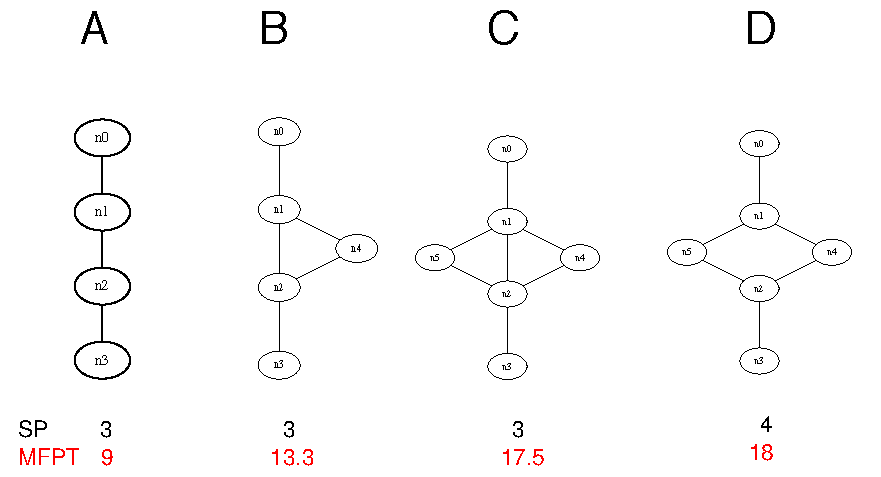
\includegraphics[width=\textwidth]{mfpt_toy.pdf}
\end{center}
\caption[Toy example of SP and MFPT on different topologies]{
{\bf Comparison of shortest path (SP) length and mean first passage time 
(MFPT) on different toy networks.}
Shown are the distances between node $n0$ and $n3$ measured in shortest path 
(SP) and mean first passage time (MFPT) respectively.
}
\label{fig:mfpt_toy}
\end{figure}

\section{Application in tumor-stroma interaction of lung cancer}

The hallmark of lung tumor development is its early spread, 
complicating the patient treatment and strongly impairing survival.
Recent studies~\citep{Mueller2004} have shown the tumor-stroma interaction to be relevant to 
tumor growth and spread, and therefore a possible target for
novel, effective treatment. 
However, 
the details by which tumor and stroma cells communicate remain poorly 
understood. In this section we present a study
of the migration mechanisms of a non-small-cell lung 
tumor cell line (H838) under the influence of endothelial (HPAEC) cells 
in a coculture system.

To obtain a holistic overview of the migratory processes, 
we recorded the time-resolved changes in the transcriptome of tumor cells
in scratch assays of aforementioned cocultures, and measured
cytokine concentrations in the medium.
H838 showed a significantly increased migration area after 24h in the 
H838/HPAEC coculture compared to the H838/H838 coculture.
Gene set enrichment test identified coordinated regulation
of transcription factors targets
that cause the transcriptome response in H838. 
We inferred the cytokines involved in the signal flow based on the 
PPI distances from the cytokine receptors to the predicted
transcription factors using both shortest path and mean first passage time.
Two cytokines, TNF-$\alpha$ and SDF-1$\alpha$, were shown to directly 
induce migration, 
and the transcripts of these two key factors were regulated only 
in HPAEC cells.
%suggests that TNF-$\alpha$ receptors activate multiple
%downstream targets in a homogeneous fashion,
%whereas the shortest paths \change[JB]{between}{descending from} 
%the SDF-1$\alpha$ receptor
%have multiple characteristic path lengths. 
%We conclude that TNF-$\alpha$ induces \change[JB]{the sustained}{an unspecific} 
%activation 
%of various downstream transcription factors, 
%which is the \change[JB]{primary}{initial} response \remove[JB]{mechanism} 
%involved in the 
%migration of H838 cells. 
%At the same time, the delayed activation of SDF-1$\alpha$ induce\change[JB]{d}{s 
%specific} pathways 
%\add[JB]{that} could provide a fail-safe mechanism.

\subsection{Background}
Lung cancer with its predominant type non small cell lung carcinoma 
(NSCLC) is the leading cause of cancer-related mortality worldwide.
The hallmark of lung cancer is its early spread, 
making it particularly dangerous, with associated high rate of death 
and short survival.
Whether this is an inherent feature of the non-small cell 
lung tumor cells or 
due to their microenvironment is still unknown. 

Ever since the formulation of the \emph{seed and soil} theory by the English 
surgeon Stephen Paget in 1889~\citep{Paget1889}, there has been increasing 
interest in studying the tumor-stroma interactions. 
It is now largely acknowledged that sites of metastasis are determined 
not only by the characteristics of the tumor
cells but also by the microenvironment of
the host tissue~\citep{Fidler2003}. Tumor cells can generate a supportive
microenvironment by producing stroma-modulating
growth factors, which act in a
paracrine manner to induce stromal reactions such as
angiogenesis~\citep{Bergers2003}
and inflammatory response~\citep{Coussens2002}. Stroma cells in turn can
interact with primary tumor cells synergistically and facilitate their migration~%
\citep{Wyckoff2004}.
Stromal cells also make promising drug targets, since they are not as 
genetically
unstable as cancer cells, and are therefore less likely to
develop drug resistance~\citep{Kerbel1997}. To date, a number of drugs targeted
at tumor microenvironment, i.e. endothelial cells, immune cells and components
of the extracellular matrix, are at different stages of clinical 
trials~\citep{Mueller2004}. However, side effects of such stroma-targeting drugs
have also been observed, which raises the natural demand of a more detailed, 
systematic understanding of the tumor-stroma interaction.

While bearing in mind that tumor-stroma interactions can be mediated by direct cell-cell contact or modification of the extracellular matrix
components~\citep{Micke2004a}, most studies have focused on the tumor-stroma interaction through
single soluble factors~\citep{Kryczek2007,Saijo2002i,Nakamura1997}. 
\cite{Zhong2008} identified cytokines that are crucial for the 
tumor cell proliferation
and stromal cell migration by screening the whole secretome from
an adenocarcinoma/stromal murine lung cell coculture.
\cite{Sato2004} studied
the transcriptome homeostasis of pancreatic
cancer cells and stromal fibroblasts,
and singled out candidate genes that are
differentially expressed in coculture.
One of the most important types of stromal cells are endothelial cells (EC), 
the integral components of blood vessels. ECs not only promote the homeostasis of 
vascular system, but play an important role in tumor progression as well. 
It was shown that ECs influence different responses of cancer cells, such as 
proliferation and invasiveness \emph{in vitro}, as well as the metastatic potential 
of tumor cells \emph{in vivo}~\citep{Franses2011}.

Here, we combine the previous approaches and
study \emph{in vitro} the crosstalk between tumor and 
endothelial cells in  a non-small-cell lung cancer model: namely,
H838 lung cancer cells and HPAEC, i.e. human pulmonary artery endothelial cells.
We found that the  migration of  H838 cells in a trans-well H838/HPAEC coculture
was significantly enhanced when compared to monoculture.
Gene set enrichment analysis of the dynamic transcriptome
response of the H838 cells  revealed a coculture specific response 
that correlated with enhanced migration.
We further 
traced causes of the transcriptome response in the tumor cells back to 
a group of sequential transcription factors.
Assuming that cellular signal is most likely transmitted through the most efficient 
path in a protein-protein interaction network, we 
mapped the putative pathways linking cytokine receptors with the 
transcription factors evoking the transcriptome response. 

Finally, a cytokine array and subsequent single factor stimulation
confirmed the cytokines \tnfa and \sdfonea
to be the main factors enhancing H838 cell migration,
being \emph{de novo} expressed and originating in the endothelial cells alone. 

%\tnfa and \sdfonea receptors. % via the transcription factors and upstream protein signaling.
%We identified the dynamic regulation pattern of transcription factors. 
%Based on \change[JB]{the above}{our results}, we hypothesize that \tnfa receptor family 
%members are likely associated with a wide spectrum of transcription factors, which
%renders the \tnfa-induced pathway an unspecific response in the first place.
%On the other hand, the \sdfonea receptor CXCR4 
%preferentially activates transcription factors such as 
%STAT3/6, LMO2, HSF1, IRF2, JUN/FOS, which are predominantly 
%enriched between 12 and 16 hours after coculture and represents a fine-tuned
%secondary activity leading to migration. \note[SD]{Should we mention the purpose of the paper in few sentences?}

% We need some concluding sentence here wraping up teh biology


% Results and Discussion can be combined.
\subsection{Results}

\subsubsection{H838 migration rate is enhanced in a transfilter co-culture with HPAEC cells}

To investigate the changes in migration behavior of lung tumor cells under the 
influence of stromal cells we cultivated  
H838 cells  together with either human pulmonary artery endothelial cells (HPAEC) or additional H838 cells in a trans-filter system (\ref{fig:migration} A).
The experimental setup (\ref{fig:h838_setup}) of the homo- and heterogeneous cocultures ensured 
similar physical and environmental conditions, thereby minimizing 
experimental artifacts, e.g. due to different cell numbers per conditions. 

Tumor cells on the bottom of the cell culture dish were scratched and the 
closing of the cell-free area was observed using time-lapse microscopy, in both
homo- and heterogenous cocultures (\ref{fig:migration} B).
In the heterogeneous cocultures, 
H838 cells close on average $963.5\pm156.8\ \mu m^2$ 
(mean $\pm$ standard deviation) within 24h, 
against $702.8\pm104.0\ \mu m^2$ in the homogeneous cocultures 
(\ref{fig:migration} C). 
% Note that we should put all these figures into one panel 
The migration area of the heterogeneous cocultures is significantly higher, and
a two-sided  $t$-test of the difference observed yields a $p$-value of 
$2.82 \times 10^{-5}$.

\begin{center}
\captionsetup{labelformat=prepage}
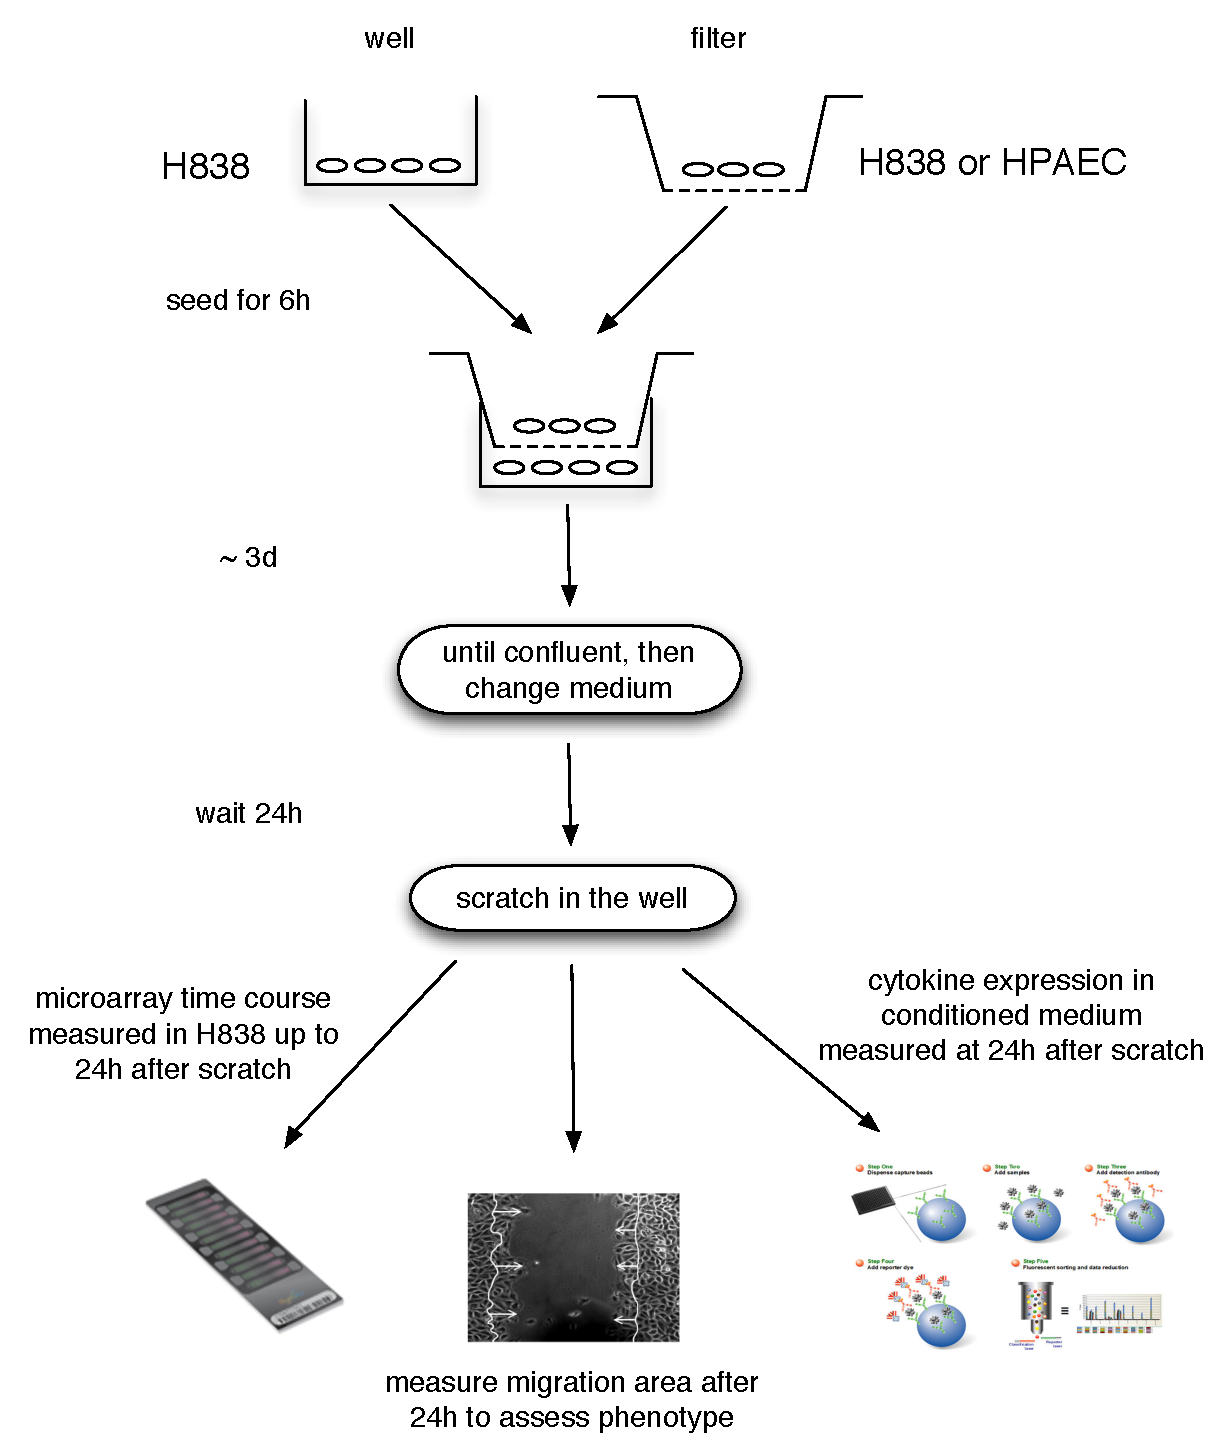
\includegraphics[width=\textwidth]{h838_setup.pdf}
\newpage
%\begin{FPfigure}[!ht]
\captionof{figure}[H838 experimental setup]{
{\bf The experimental setup of the tumor-stroma interaction 
between H838 and HPAEC cells.} 
The coculture of tumor and endothelial cells is carried out
in a trans-filter system, where the lung cancer cell line
H838 is cultivated in a well and on top of that is a filter
with either the same tumor cells or the endothelial cell
line HPAEC. Both cell types are seeded for 6 hours before 
the well and the filter are brought together. After 
approximately 3 days of coculture and both the well and the 
filter layers become confluent, medium is changed. Then
after another 24 hours, multiple scratches are performed
in the bottom well. Migration phenotype is measured within
24 hours after scratch and the cell and supernatant samples 
are subject to the transcript and cytokine profiling 
experiments respectively.
}
\label{fig:h838_setup}
%\end{FPfigure}
\end{center}

\begin{figure}[!ht]
\begin{center}
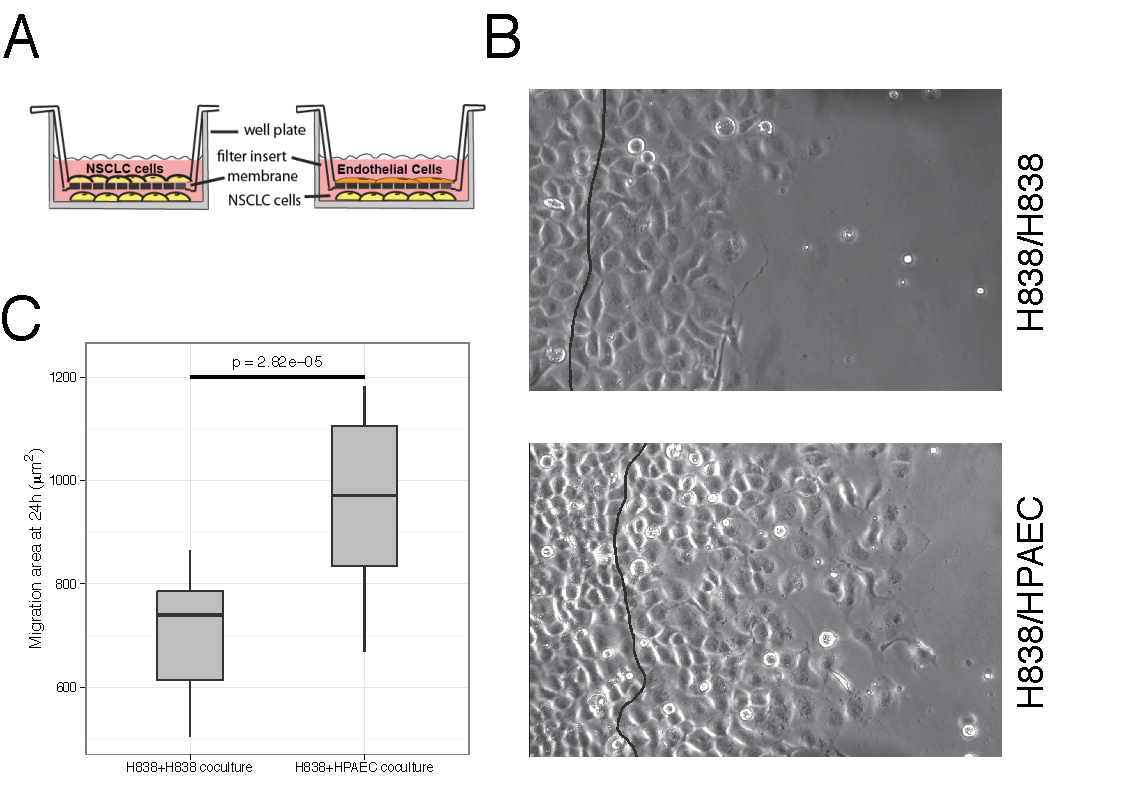
\includegraphics[width=\textwidth]{fig-migration.pdf}
\end{center}
\caption[H838 migration in homo- and heterogeneous coculture]{
{\bf Migration of H838 cells in the homo- and heterogeneous coculture.} 
(A) Trans-filter system. (B) Scratch assay of the homo- and heterogeneous coculture.
(C) Migration area of H838 cells at 24h after scratch from multiple independent 
experiments 
plotted as 
boxplots for the homogeneous (H838 + H838) and heterogeneous (H838 + HPAEC) 
coculture.
}
\label{fig:migration}
\end{figure}

The \emph{in vitro} scratch assay is a well established method
to study cell migration~\citep{Busch2008,Liang2007}, especially
in our experimental setting, the coculture of tumor and 
endothelial cells has no influence on the cell proliferation~%
\citep{Dauscher2012} and thus our results can be interpreted
as the net effect of tumor cell migration.

\subsubsection{Transcriptome response of H838 cells}
To explore the mechanisms leading to the enhanced cell migration, we recorded the time-resolved transcriptome response of the tumor cells during migration.
Illumina Human HT-12 Expression BeadChip was employed to compare the dynamic transcriptome response of scratched H838 cells in both homo- and heterogenous coculture conditions.
We collected mRNA at $t=(0,0.5,1,2,3,4,5,10,15,24)h$ after scratching for microarrays,
the data of which were quantile-normalized~\citep{Dunning2008a}.  
Discarding lowly expressed probesets and those with low interquartile 
variability between samples, we finally mapped the probes to 14922 EntrezID 
annotated genes. 
% Here we should show a time-resolved GO analysis or something similar (Fig. 2)
% Also add the analysis in the materials and methods

We analyzed the basal differential gene expression between homo- and
heterogeneous coculture by linear model fitting and Bayesian variance estimation~%
\citep{Smyth2004}, as well as the dynamic differential gene expression by fitting
the time series with a full/reduced polynomial model~\citep{Mar2009}. At 0h, only 2
genes are significantly down-regulated (Benjamini-Hochberg
corrected $p$-value $<0.01$) in the homogeneous coculture with respect
to the heterogeneous coculture 
(\ref{fig:h838_transcriptome} A). Over time, there are more
genes classified as significantly up- and down-regulated by comparing the full and
reduced model fitting (\ref{fig:h838_transcriptome} B). 
We further looked at the time course of all genes that are
significantly ($q<0.01$) regulated over time from 
\ref{fig:h838_transcriptome} B. In the heterogeneous
coculture of H838 and HPAEC cells, most genes are 
moderately up-regulated over time, with the maximal
log fold expression being 1.25 relative to 0h.
Taken together, the majority of genes
in H838 cells are not differentially expressed in the homo- and heterogeneous
coculture conditions. We hypothesize that those 
differentially regulated genes do contribute to certain specific
phenotypic transformations, but the response of the H838
transcriptome to heterogeneous coculture is rather weak.

\begin{figure}[!ht]
\hskip 0.5in A \hskip 2.5in B
\begin{center}
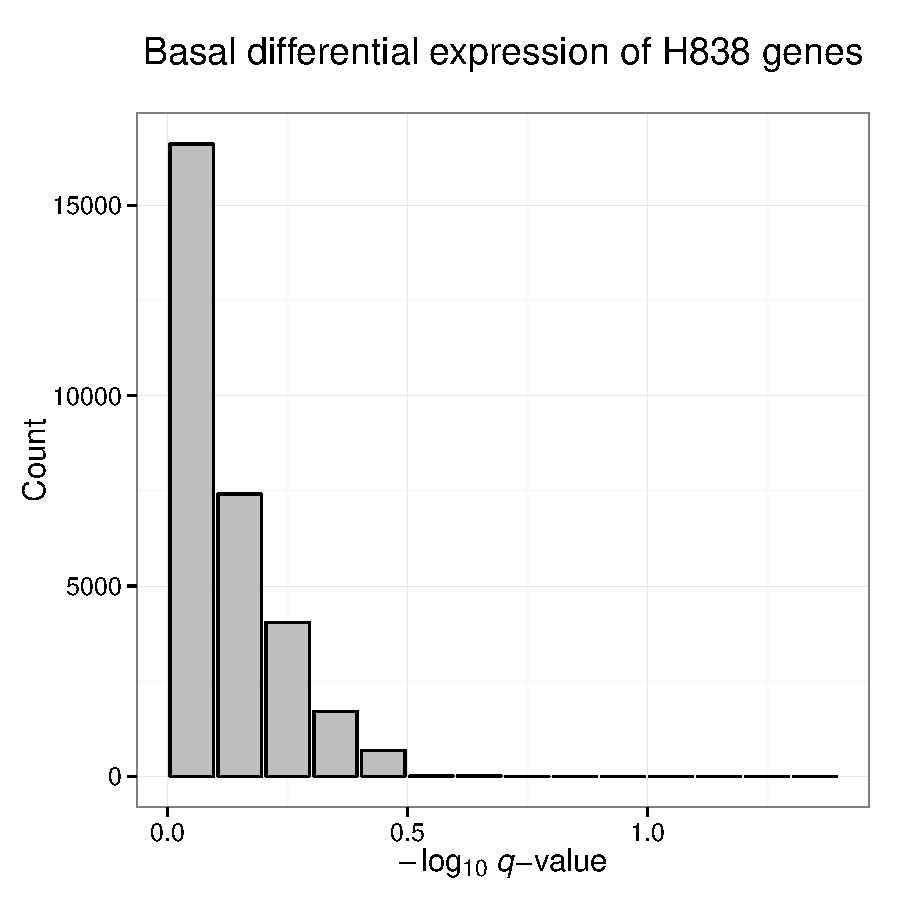
\includegraphics[width=0.45\textwidth]{h838-basal_hist.pdf}
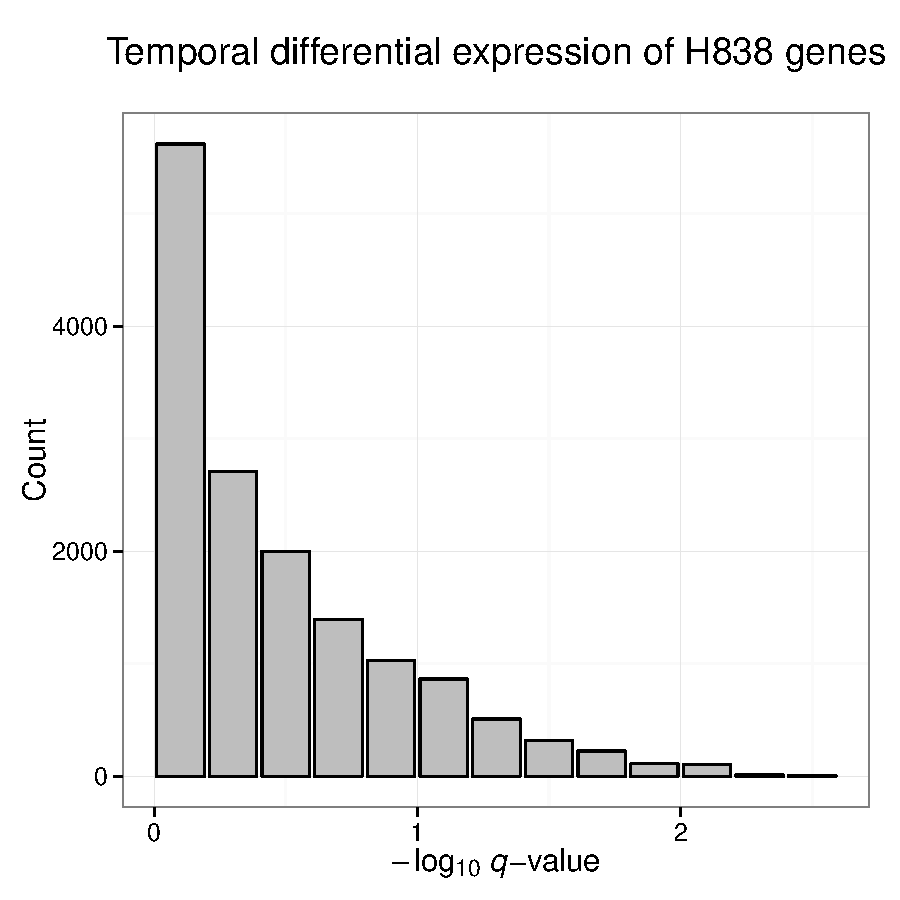
\includegraphics[width=0.45\textwidth]{h838-fit_hist.pdf}
\end{center}
\caption[Differential basal and dynamic gene expression]{
{\bf Differential basal and dynamic gene expression in homo- and heterogeneous 
cocultures.} 
(A) Histogram of the differential gene expression at 0h as determined by limma~%
\citep{Smyth2004}. 
Basal differential expression is 
represented as the negative log-transformed and multiple
testing corrected $p$-value of the limma test.
(B) Histogram of the differential gene expression over time as determined by the
full/reduced model fitting~\citep{Mar2009}.
Dynamical differential expression is 
represented as the negative log-transformed and multiple
testing corrected $p$-value of the full/reduced model
likelihood ratio test.
}
\label{fig:h838_transcriptome}
\end{figure}

\begin{figure}[!ht]
\begin{center}
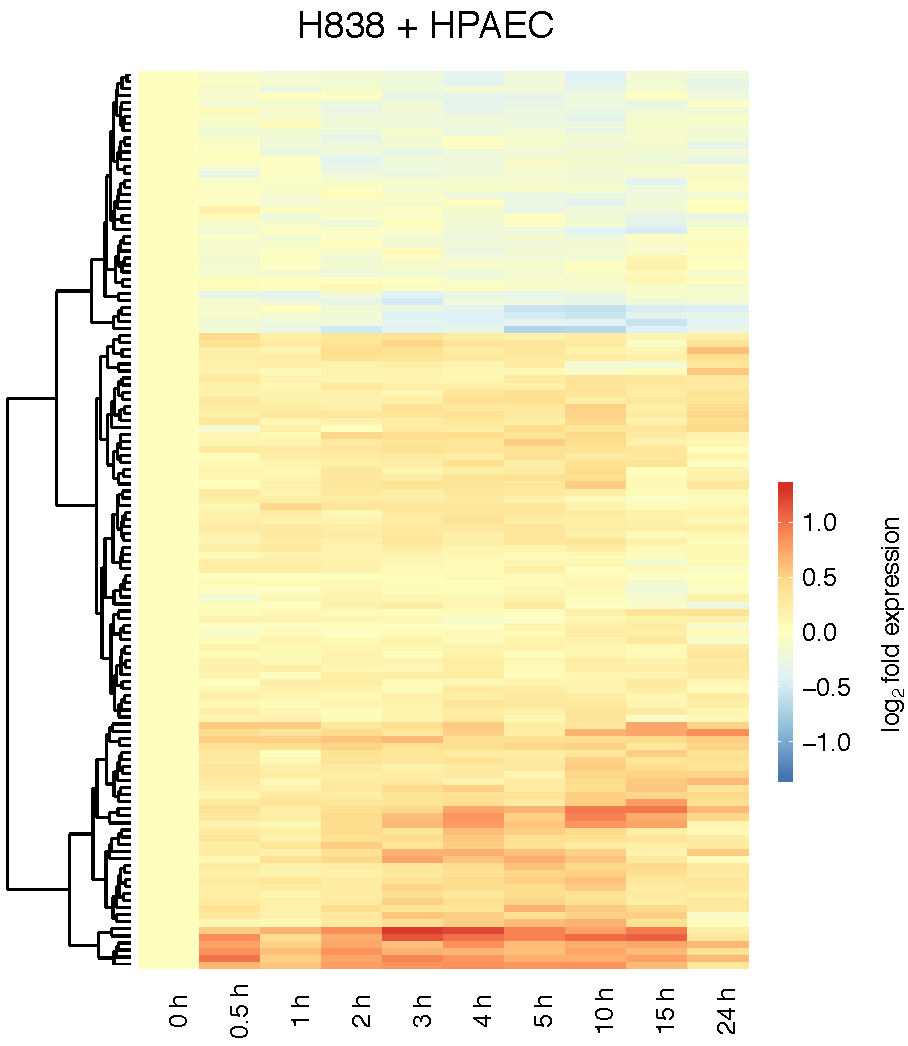
\includegraphics[width=\textwidth]{h838_ts_heatmap.pdf}
\end{center}
\caption[Gene expression time course in the H838/HPAEC coculture]{
{\bf Time course of significantly regulated genes in the H838/HPAEC heterogeneous coculture.} 
Color code is the normalized log fold expression relative to 0h, a hierarchical
clustering dendrogram of the time series is shown to the left.
}
\label{fig:h838_ts}
\end{figure}

In order to take a glance at what is the function of those
differentially regulated genes, and to overcome the difficulty in detecting weak
but simultaneous regulation, we analyzed the transcriptome data with gene set
enrichment test~\citep{Luo2009}.
The comparison between heteregeneous and homogeneous coculture yields 
a mixture of experimentally determined gene sets, both for the basal level
(\ref{fig:h838_basal_gage_msigdb})
and the differential expression over time (\ref{fig:h838_dynamic_gage_msigdb}).
In other words, the H838 cells in the heteregeneous and homogeneous coculture
do not tend to have a qualitatively different phenotype and are migrating in
both cases as is also observed in the scratch assay.

\begin{figure}[!ht]
\begin{center}
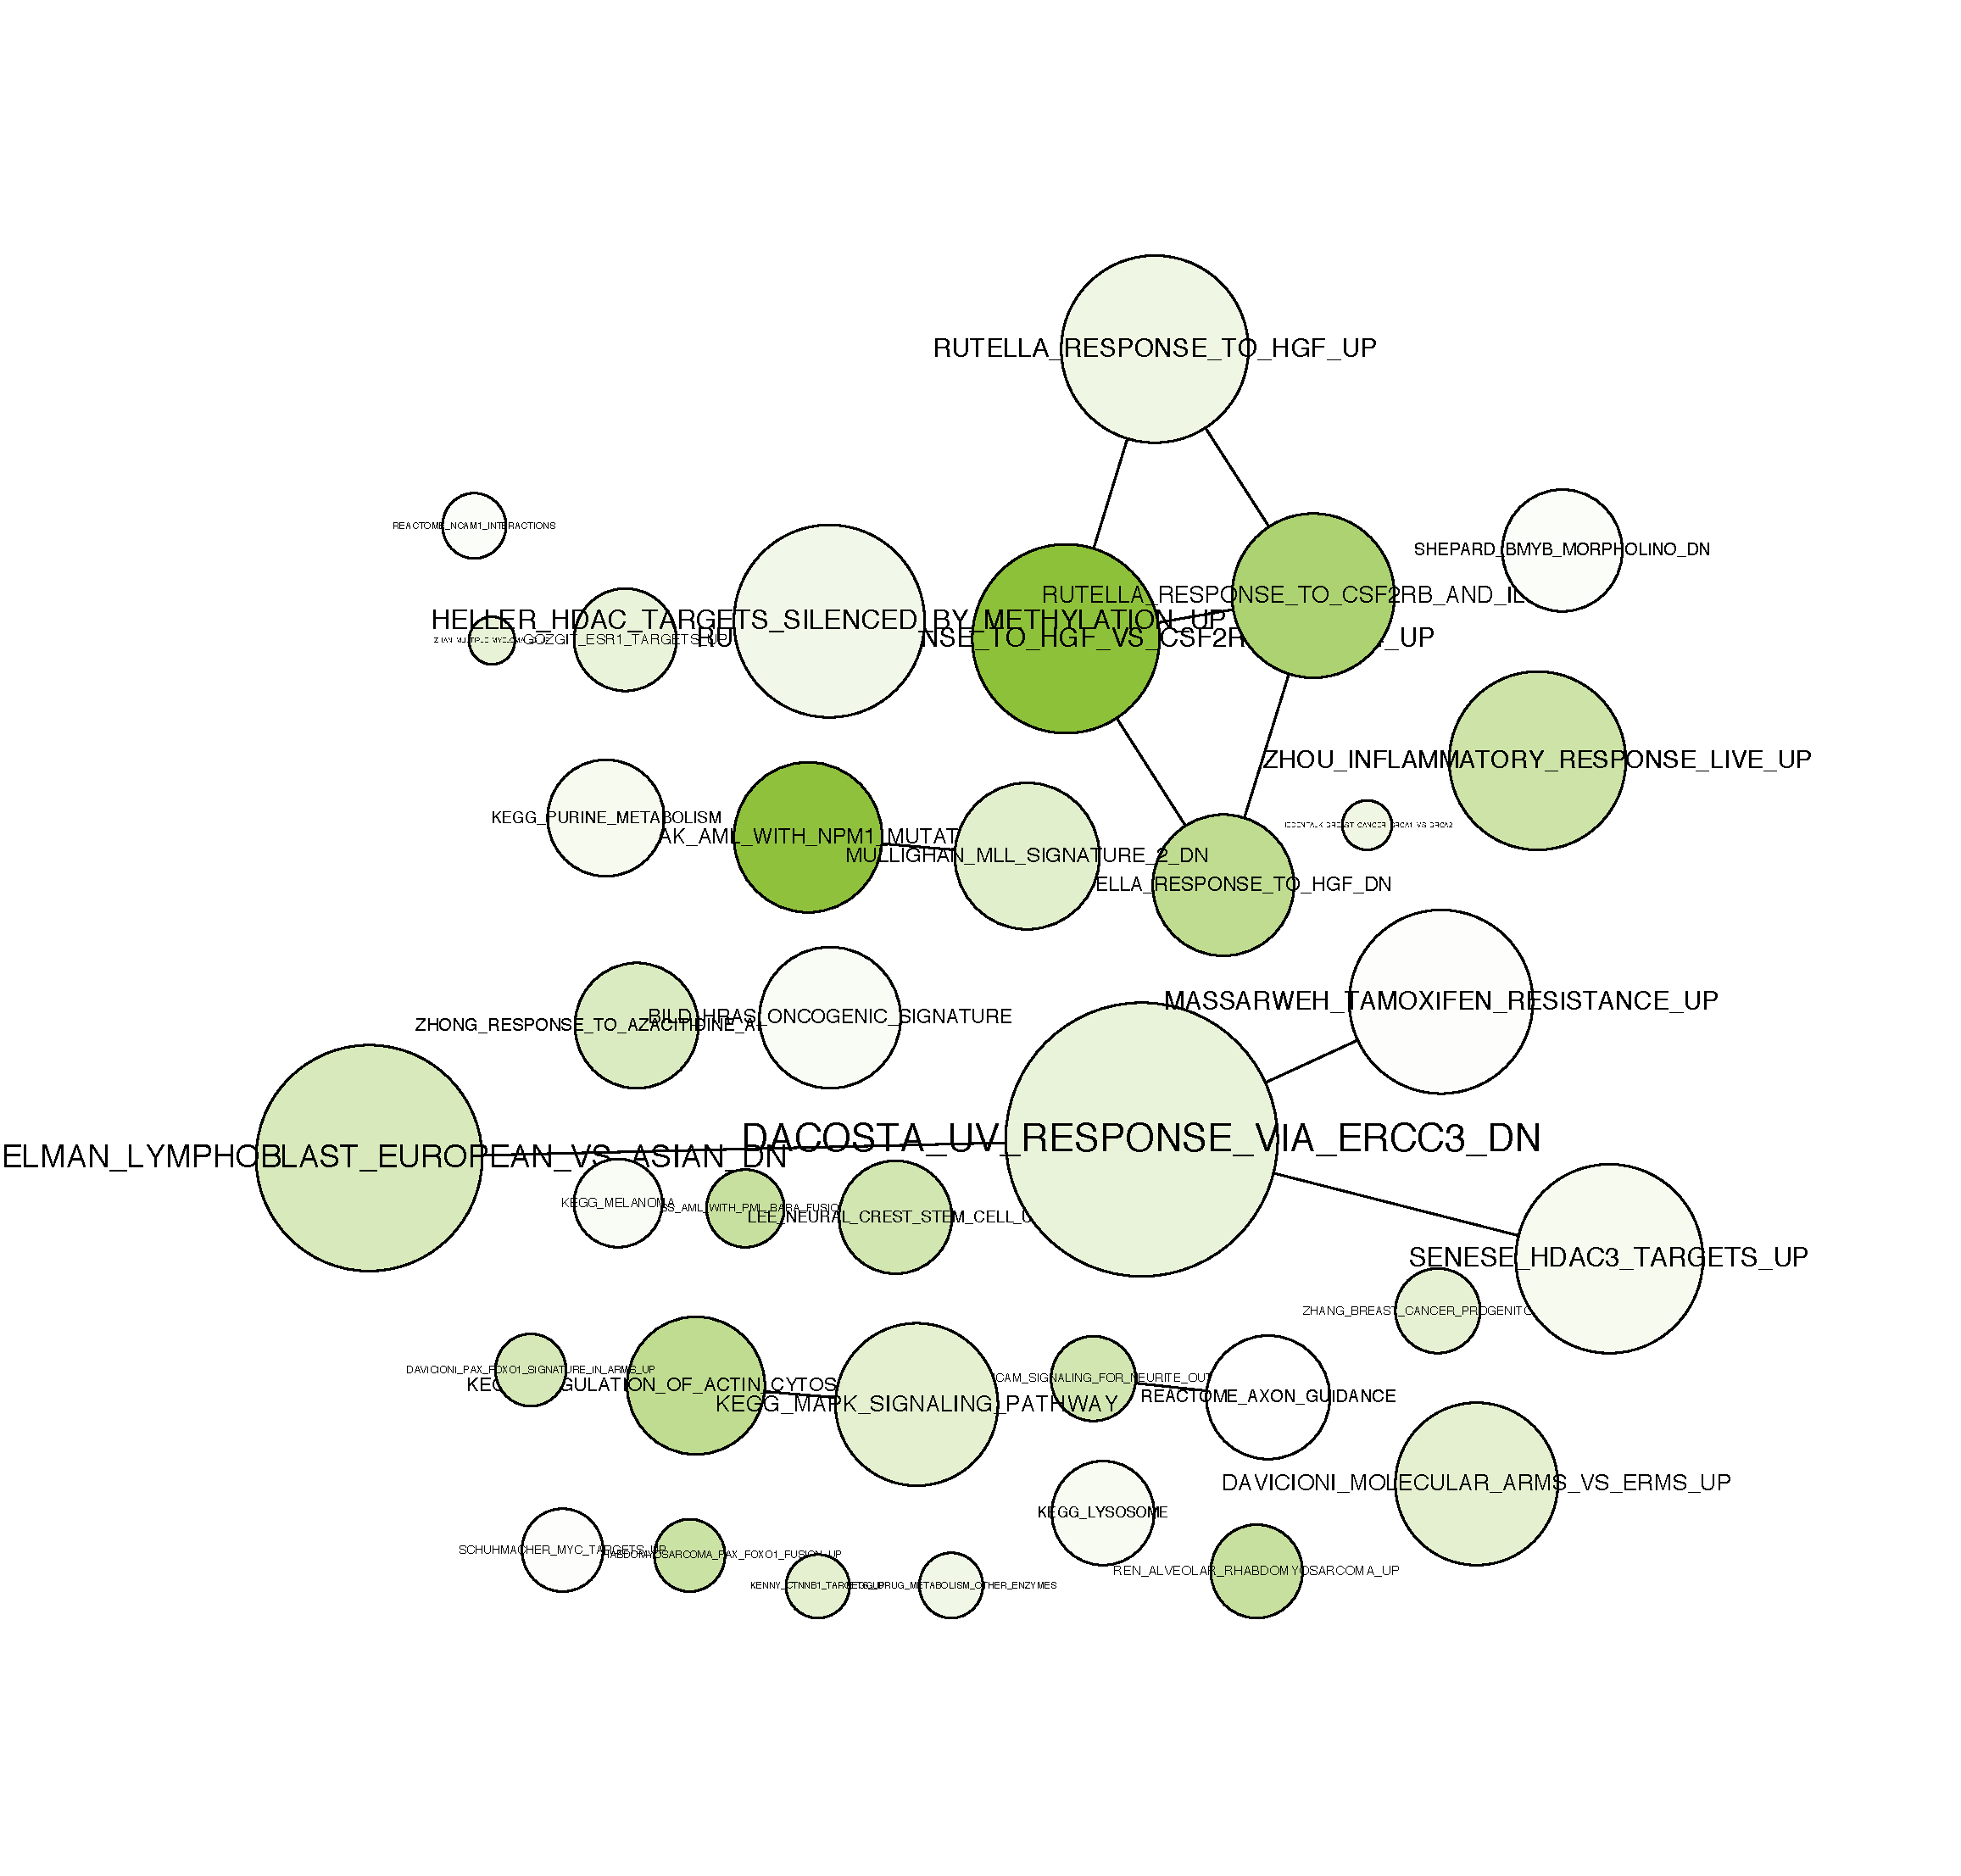
\includegraphics[width=\textwidth]{h838_basal_gage_msigdb.pdf}
\end{center}
\caption[Basal gene set enrichment]{
{\bf Basal gene set enrichment between heterogeneous and homogeneous cocultures.} 
The fold changes between heterogeneous and homogeneous coculture expressions 
for a certain gene set at 0h are compared with the background using $t$ test.
The signicance level (negative log-transformed $p$-value) is color-coded, such
that green means enrichment of a gene set and white means depletion. The size
of the gene set is coded by the size of the circles.
}
\label{fig:h838_basal_gage_msigdb}
\end{figure}

\begin{figure}[!ht]
\begin{center}
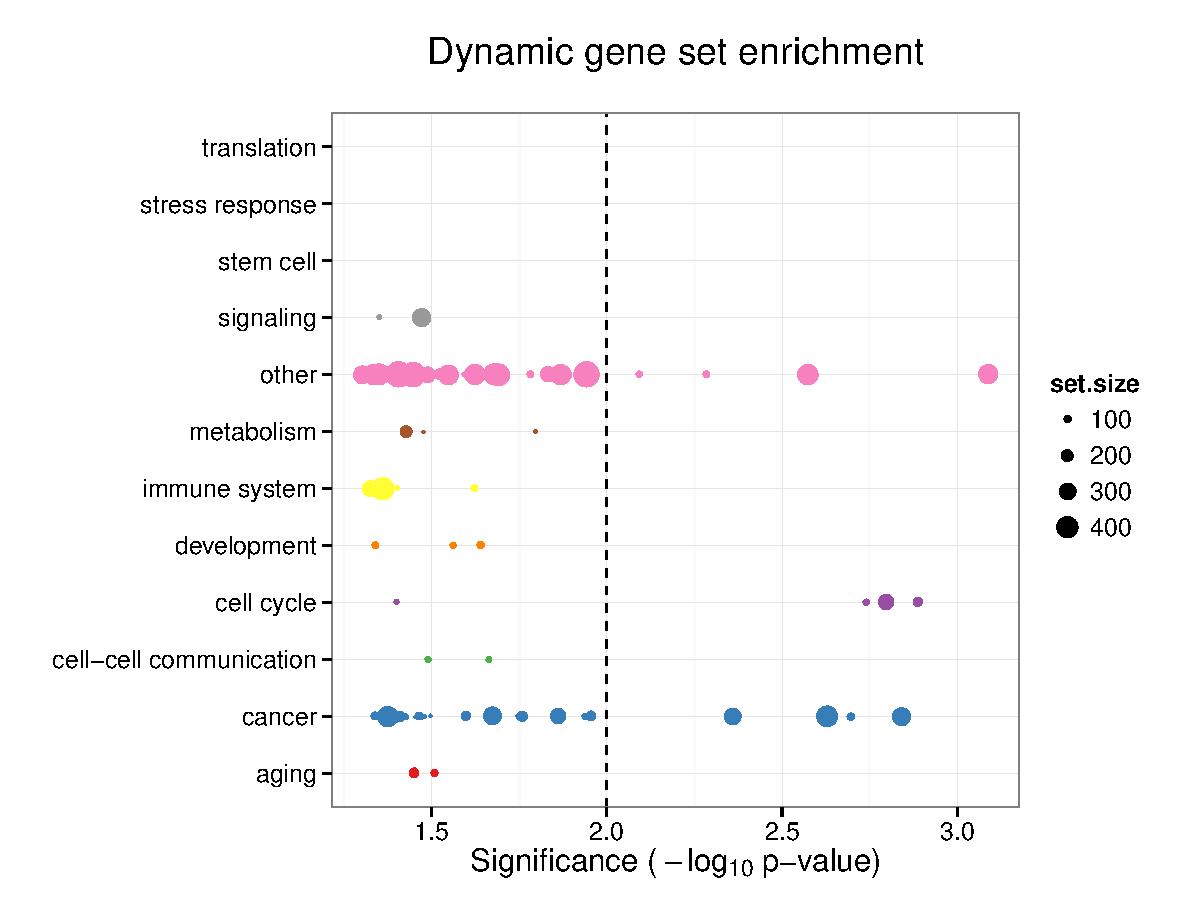
\includegraphics[width=\textwidth]{h838_dynamic_gage_msigdb.pdf}
\end{center}
\caption[Dynamic gene set enrichment]{
{\bf Dynamic gene set enrichment between heterogeneous and homogeneous 
cocultures.} 
The differential expression of each gene is first assessed by the full/reduced
model (\ref{sec:full_reduced}), the mean differential score of a gene set
is then compared with that of the background set using $t$ test.
The signicance level (negative log-transformed $p$-value) is color-coded, such
that green means enrichment of a gene set and white means depletion. The size
of the gene set is coded by the size of the circles.
}
\label{fig:h838_dynamic_gage_msigdb}
\end{figure}

The functional association of the transcriptome response, however, can be
decoded in a fine-tuned gene set enrichment test between the 0h unscratched
sample and each of the other time points. In the heteregeneous coculture 
(\ref{fig:h838_hetero_gage}),
we see an initial enrichment of gene sets related to breast cancer, terms
such as metastasis are over-represented between 1 and 2 hours, which are
again followed by cell migration related gene sets at 4h. After 5 hours,
the functions of enriched gene sets diverge and become less specific.
In contrast, although the enriched gene sets of homogeneous coculture also 
include cancer-related terms, there is no visible general trend that can
be followed over time (\ref{fig:h838_homo_gage}). 

\begin{figure}[!ht]
\begin{center}
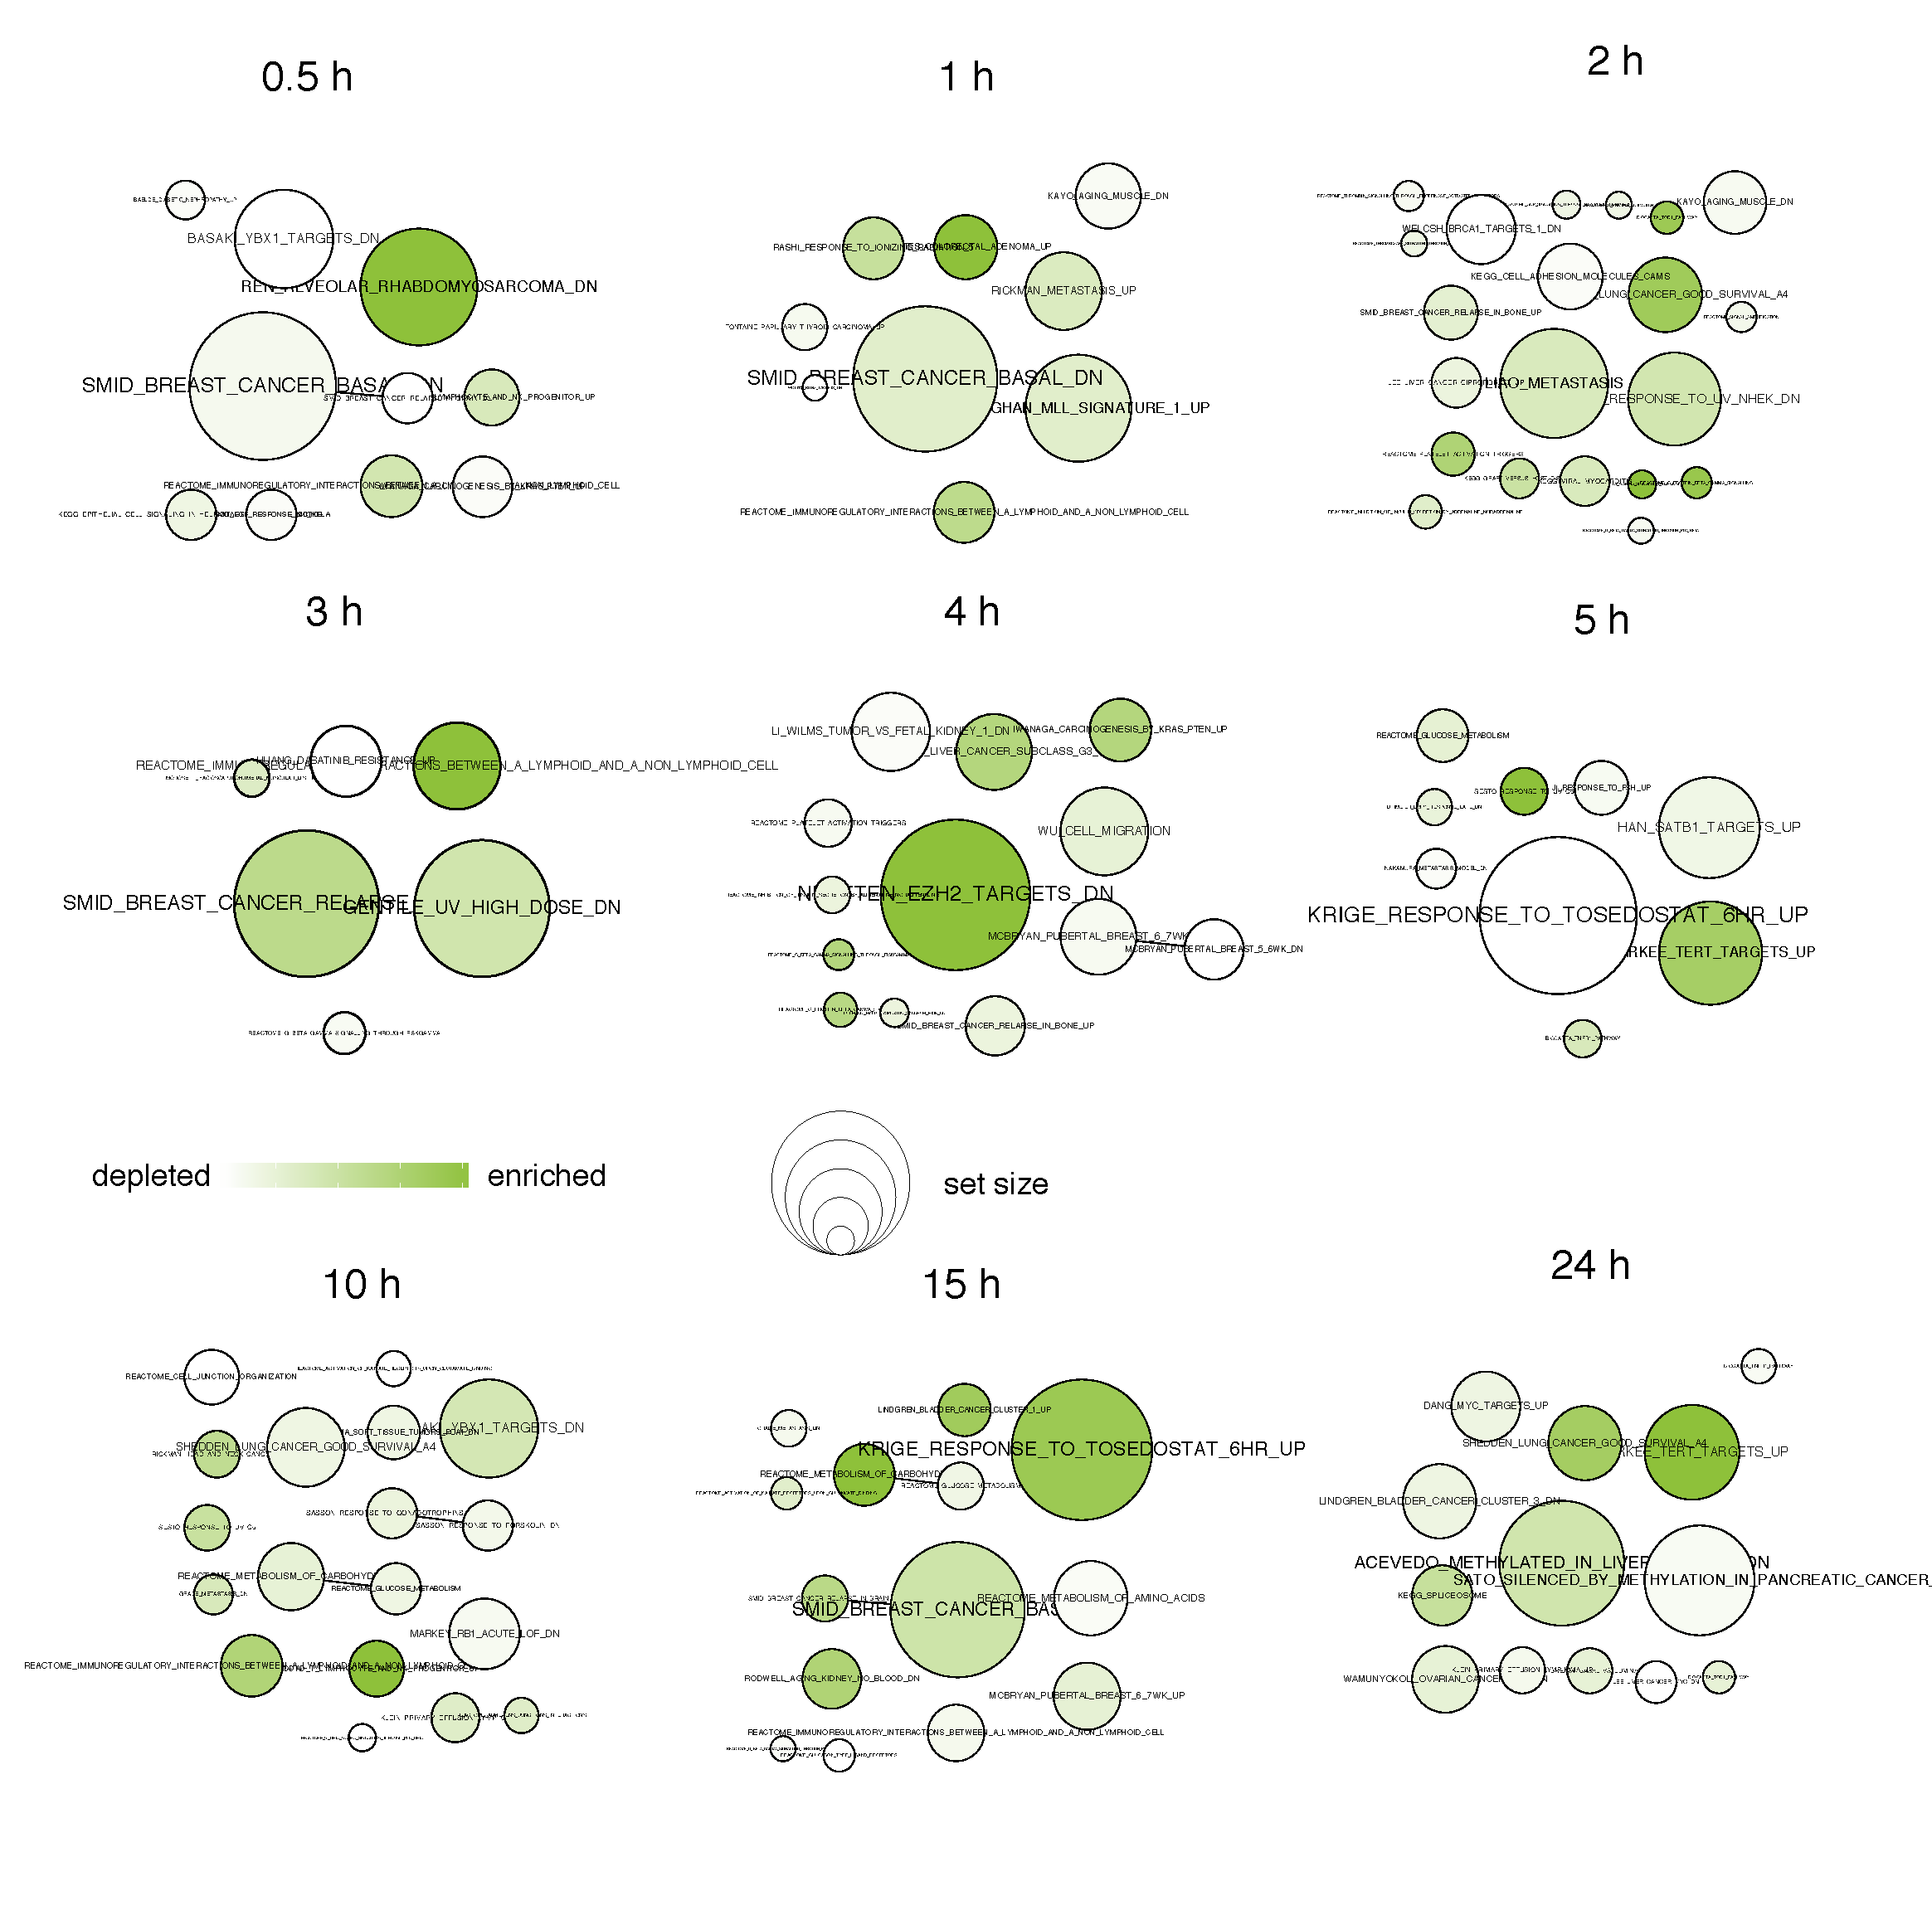
\includegraphics[width=\textwidth]{h838_HMEC_gage.pdf}
\end{center}
\caption[Gene set enrichment of the heterogeneous coculture]{
{\bf Gene set enrichment between different time points and 0h in the heterogeneous 
coculture.} 
The differential expression of each gene is first assessed between time points, 
the mean differential score of a gene set
is then compared with that of the background set using $t$ test.
The signicance level (negative log-transformed $p$-value) is color-coded, such
that green means enrichment of a gene set and white means depletion. The size
of the gene set is coded by the size of the circles.
}
\label{fig:h838_hetero_gage}
\end{figure}

\begin{figure}[!ht]
\begin{center}
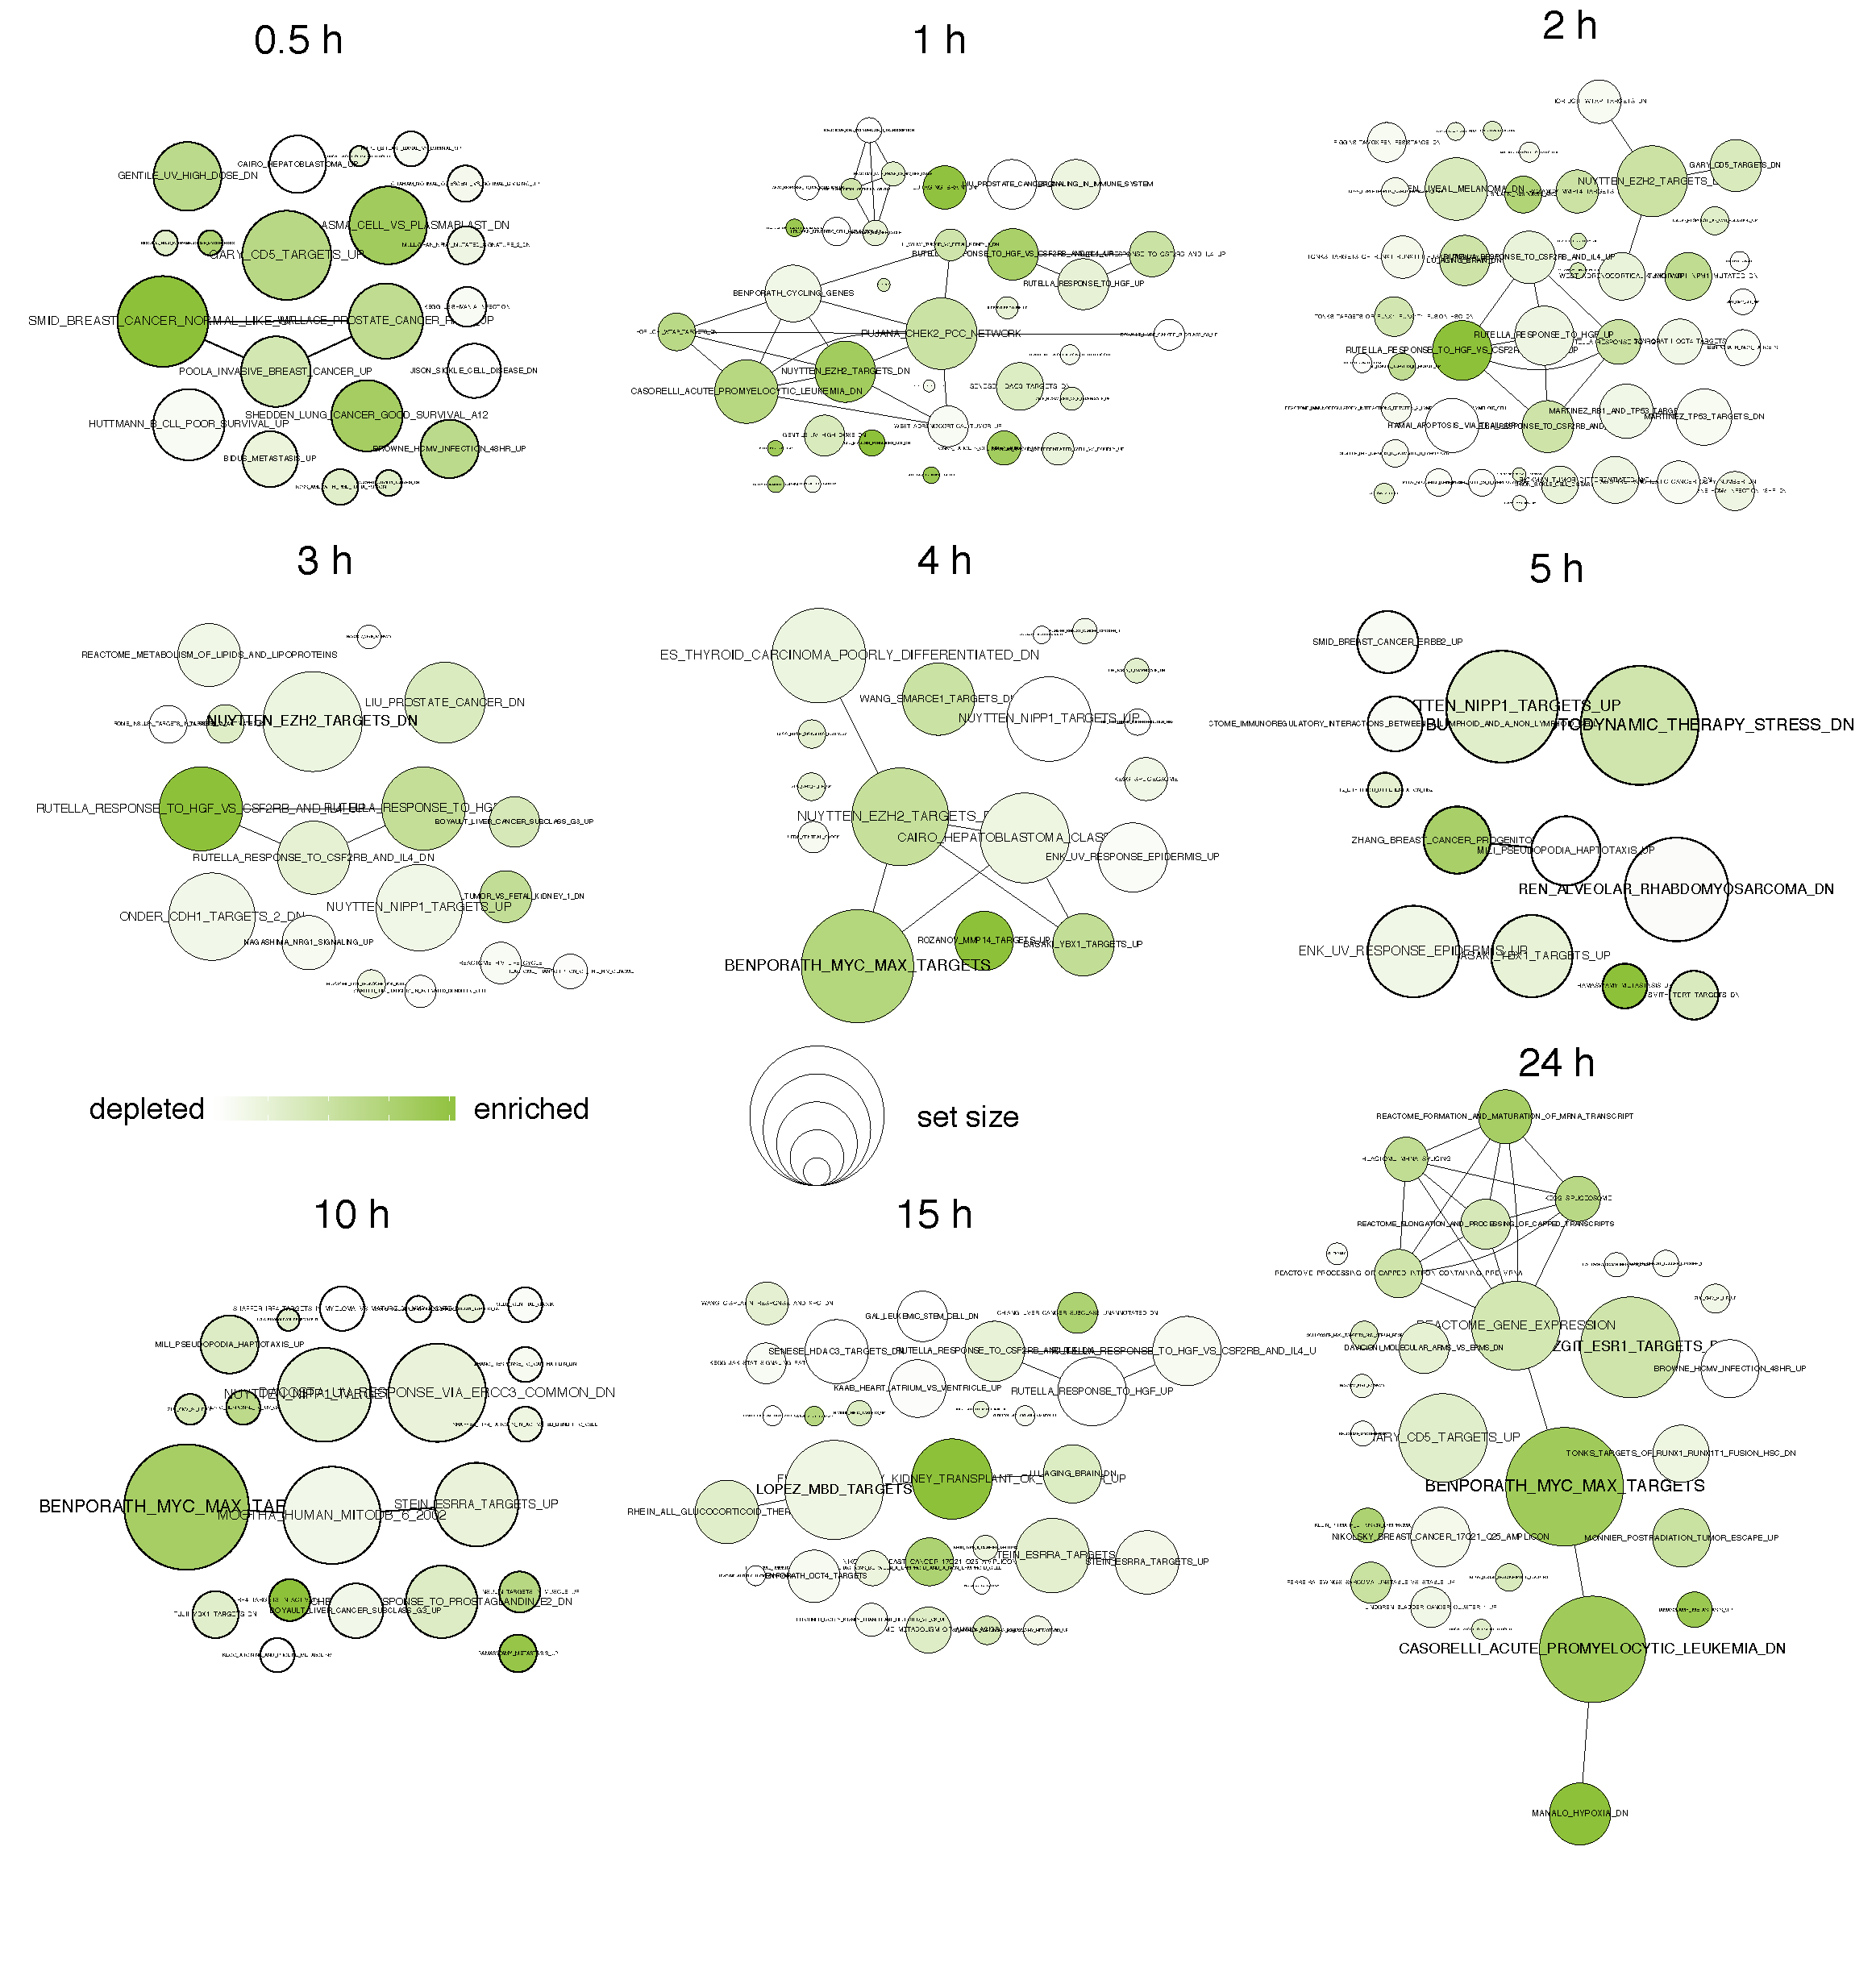
\includegraphics[width=\textwidth]{h838_Mono_gage.pdf}
\end{center}
\caption[Gene set enrichment of the homogeneous coculture]{
{\bf Gene set enrichment between different time points and 0h in the homogeneous 
coculture.} 
The differential expression of each gene is first assessed between time points, 
the mean differential score of a gene set
is then compared with that of the background set using $t$ test.
The signicance level (negative log-transformed $p$-value) is color-coded, such
that green means enrichment of a gene set and white means depletion. The size
of the gene set is coded by the size of the circles.
}
\label{fig:h838_homo_gage}
\end{figure}

We further investigated
the enrichment of KEGG pathways for both heterogeneous and homogeneous 
coculture (\ref{fig:h838_gage_kegg}). By grouping the time points into 3 
consecutive phases (early,
intermediate, late), we can identify the MAPK signaling pathway as a prominent 
candidate in the heteregeneous coculture. The MAPK pathway also shares 
member proteins with other pathways, as indicated by the edges in 
\ref{fig:h838_gage_kegg}, which hints at the possibility of the MAPK pathway
crosslinking with other signaling pathways.\footnote{We also discuss this
result later in detail.} On the other hand, a number of different pathways 
are over-represented in the homogeneous coculture, whereas the MAPK
pathway is absent.

\begin{figure}[!ht]
\begin{center}
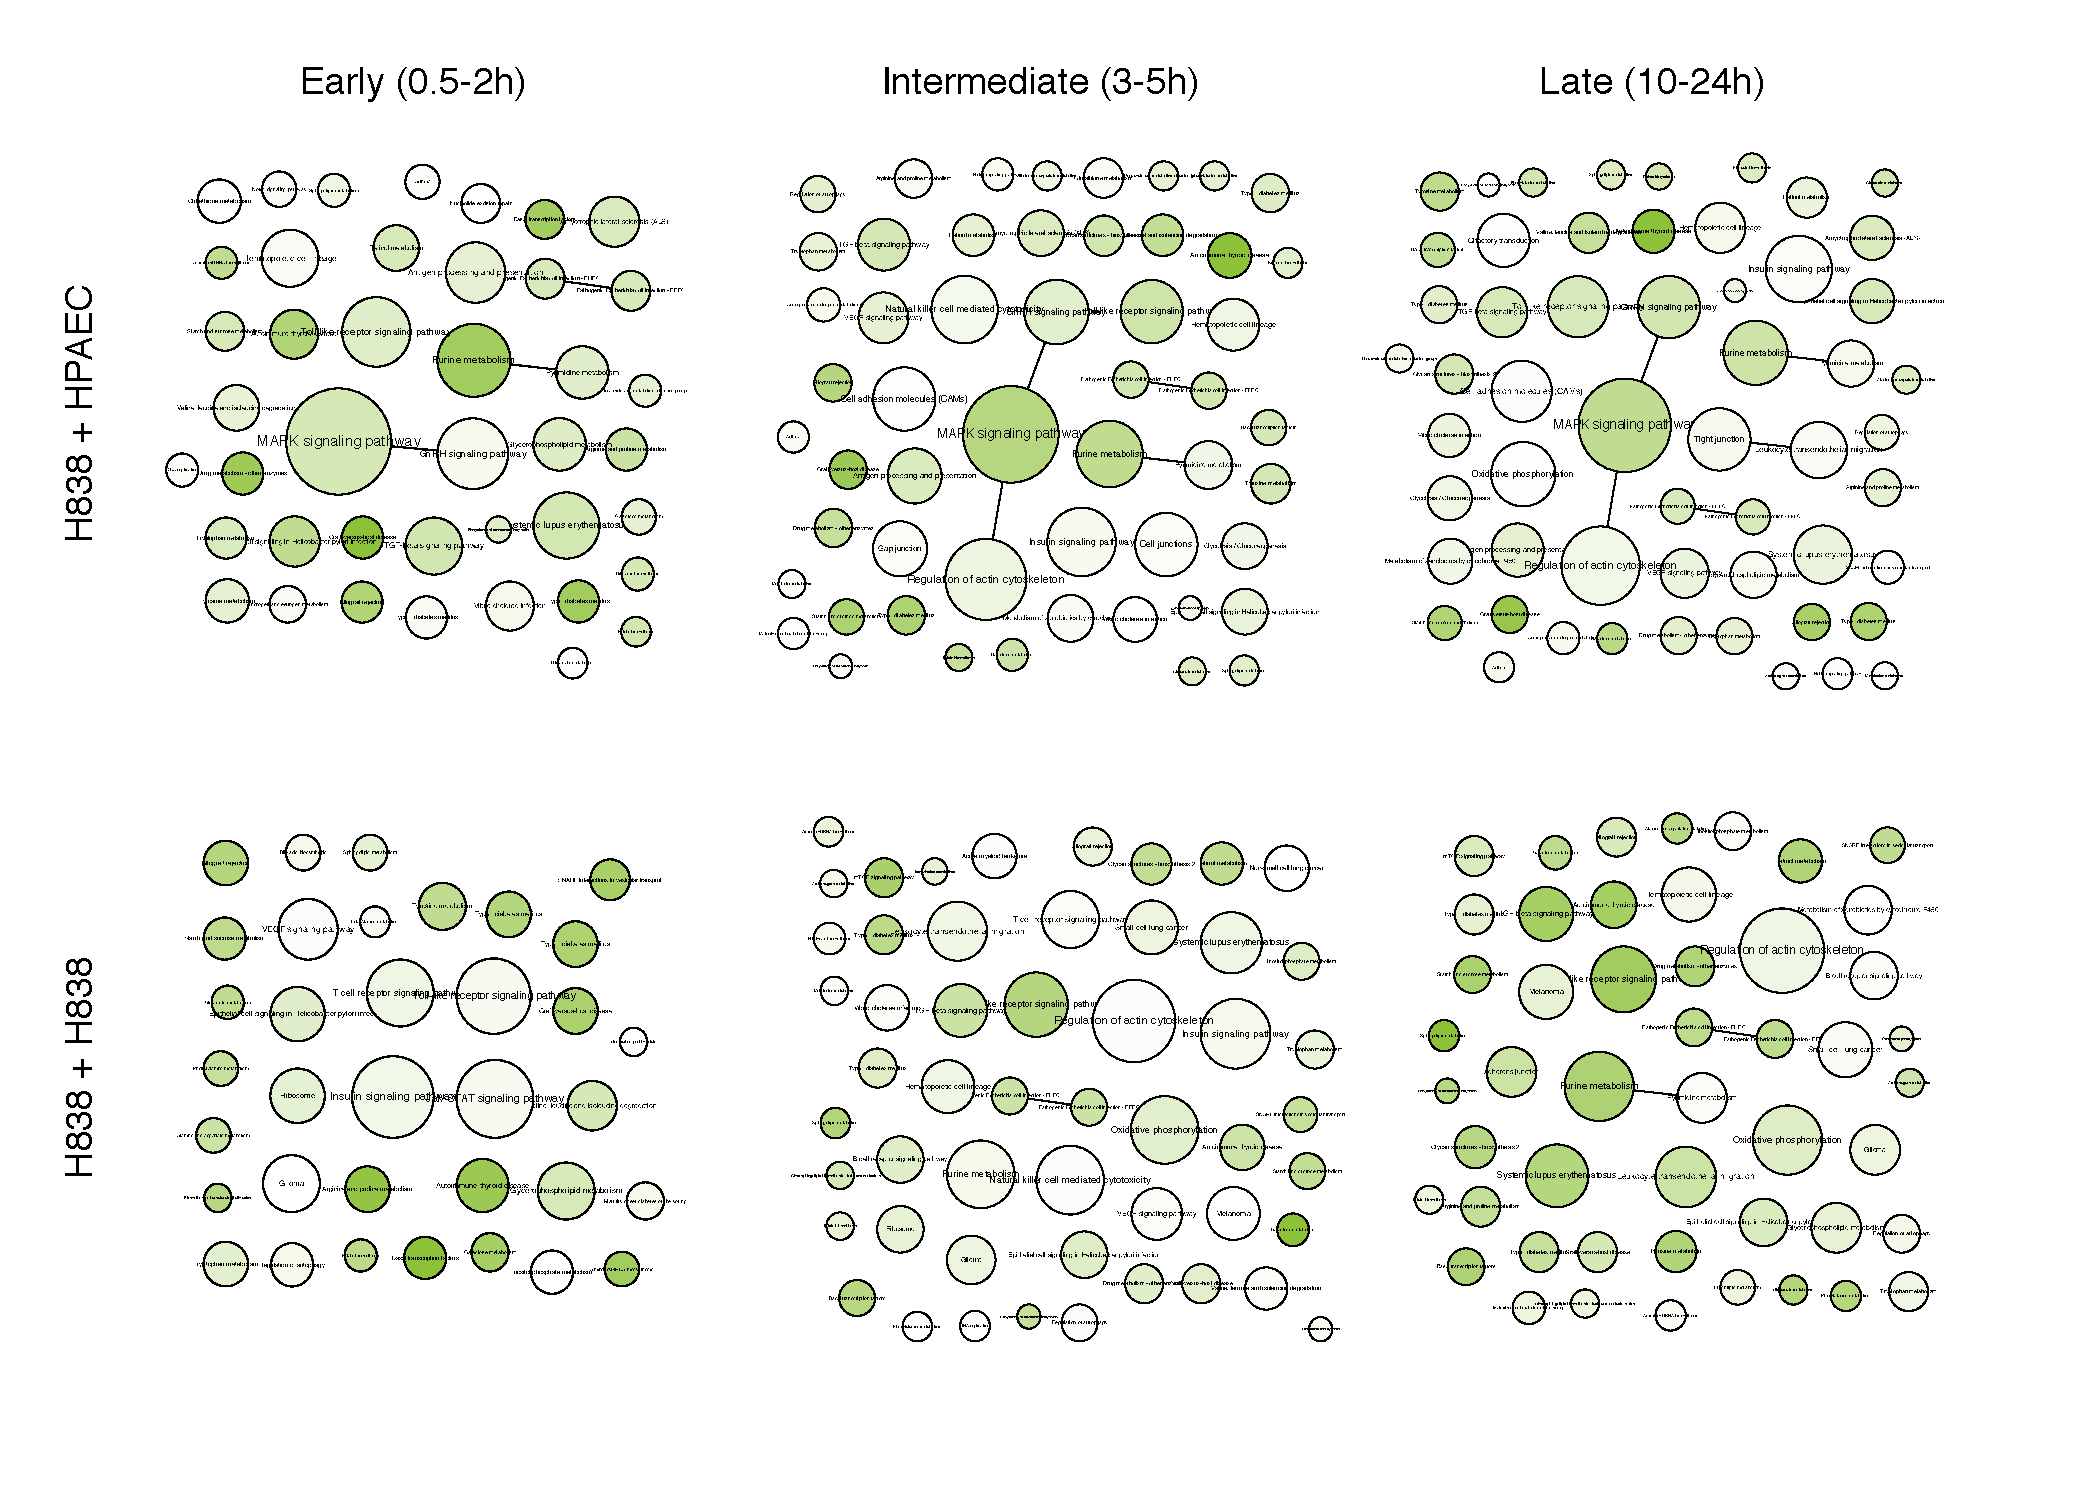
\includegraphics[width=\textwidth]{h838_gage_kegg.pdf}
\end{center}
\caption[KEGG pathway enrichment]{
{\bf KEGG pathway enrichment of the heterogeneous and homogeneous 
cocultures in three phases.} 
The differential expression of each gene of different time phases is first 
compared to 0h, the mean differential score of a KEGG pathway
is then compared with that of the background set using $t$ test.
The signicance level (negative log-transformed $p$-value) is color-coded, such
that green means enrichment of a gene set and white means depletion. The size
of the KEGG pathway is coded by the size of the circles.
}
\label{fig:h838_gage_kegg}
\end{figure}

\subsubsection{Identification of putative transcription factors in the H838 gene regulation}

The cellular signal flow, in the form of pathway activation
downstream from membrane receptors and the subsequent 
transcriptional 
regulation, is made non-trivial by the fact that proteome 
and transcriptome regulation changes have different time scales~\citep{Busch2008}. 
To overcome this difficulty, we infer the signal flow by 
tracing the cause of the transcriptome dynamics back to the external stimuli via putative transcription factors, protein-protein interaction
and receptor activation. 

We first applied a gene set enrichment test for the gene expression at 
the different time points using the transcription factor target gene sets (The Molecular Signature Database).
For each time point, 
genes were ranked according to their fold expression values
between the homo- and heterogenous coculture responses. 
A $t$-test is subsequently performed for each
transcription factor target gene set at a certain time 
point compared to the 
background set.

All significantly ($p$-value $<0.05$) enriched 
transcription factors at individual time points are 
depicted in \ref{fig:h838_tf}. Up to 2 hours, nuclear
factor family, AP-1 complex (JUN, FOS) and other diverse
transcription factors are active and responsible for 
inducing immediate early genes. Between 3 and 4 hours after
scratch, several E2F and E4F transcription factors take
over the control and effectively become the secondary 
transcriptional regulators. Active transcription factors
at later time points are less in number than the early 
active ones.
Taken together, applying the gene set
enrichment method on the time-resolved microarray data, we identified here the
sequence of putatively enriched transcription factor targets, which could also serve as
a proxy for the temporal activity of transcription factors \emph{per se}.

\begin{figure}[!ht]
%\newpage
\begin{center}
%\captionsetup{labelformat=prepage}
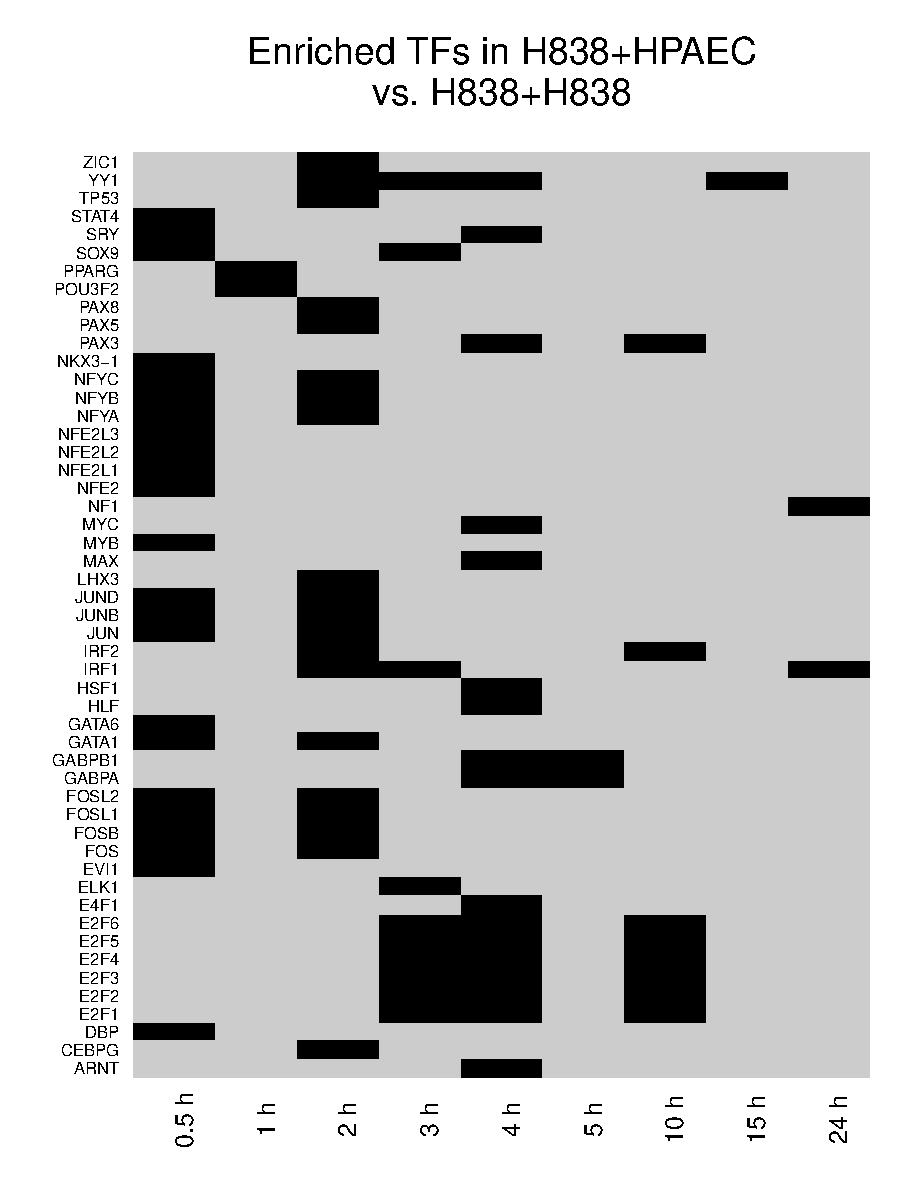
\includegraphics[width=0.8\textwidth]{h838-tf_heatmap.pdf}
\end{center}
\caption[Enrichment of transcription factors]{
{\bf Enrichment of transcription factor target genes in
the H838 cells cocultured with HPAEC at each time point.} 
Black squares indicate the over-representation ($p<0.05$) of the  
target genes regulated by a particular transcription factor
at a given time point, while gray squares indicate the
absence of such enrichment.
}
\label{fig:h838_tf}
\end{figure}

\subsubsection{Data-mining the pathways from cytokine receptors to transcription factors and gene response}

To further bridge the gap between the transcription factors identified above and the membrane cytokine receptors that 
transmit the external signal,
we mapped the most likely paths from each cytokine receptor to all putative 
transcription factors, using the HIPPIE network~\citep{Schaefer2012} and a 
distance metric based on random walk.

In order to justify the information in the PPI network, we want to prune the
raw interaction network to a smaller
high-quality one. At the same time, we also want to keep as 
much information as possible. In \ref{fig:h838_component}, we prune the 
network with different cutoff values in the confidence score for a particular
interaction. After pruning, the
size of the largest connected component first stays constant with the increase 
of the cutoff and then drops
sharply at a cutoff value of 0.6. As a trade-off, we choose to prune the PPI network
to only have interactions with a confidence score $>0.6$ such that the data
are reasonably reliable and the size of the network is also not too small to
gain insights into the signal flow between receptors and transcription factors.

\begin{figure}[!ht]
\begin{center}
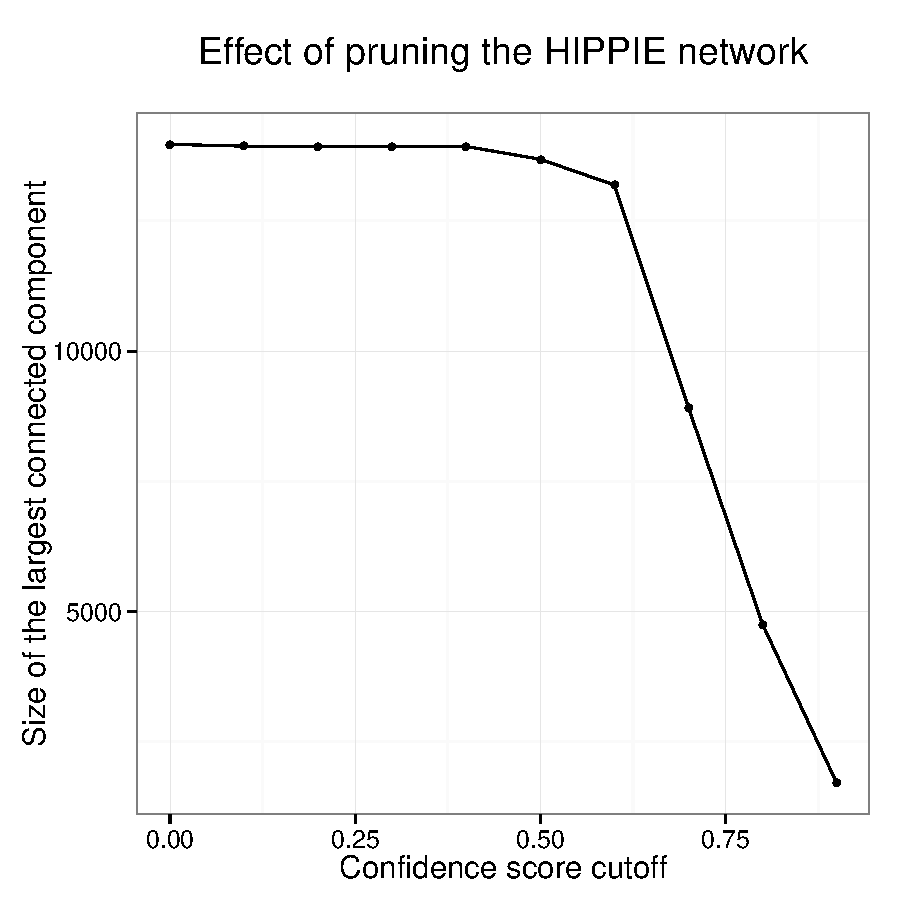
\includegraphics[width=0.7\textwidth]{h838-component.pdf}
\end{center}
\caption[Confidence score cutoff]{
{\bf Size of the largest connected component decreases with the confidence
score cutoff.} 
The size of the largest connected component in a pruned HIPPIE network decreases
with the increase of the confidence score cutoff value.
}
\label{fig:h838_component}
\end{figure}

We further want to compare both shortest path length (SP) and mean first 
passage time (MFPT) as a distance metric to infer the dynamic signal flow
in the network from receptors to transcription factors. To this end, we
first determined at eacj time point for each receptor its nearest transcription factor (with
the shortest distance metric), this distance metric for a certain receptor
$i$ is then $z$-transformed, such that both are comparable, or
\[
\tilde{D}_{i} = \frac{D_{i}-\mu(D)}{\sigma(D)}, 
\]
where $D \in \{SP,MFPT\}$ and $\mu$ and $\sigma$ are the population mean and 
standard deviation respectively. In \ref{fig:h838_mfpt_sp}, we see the median
statistics of both distance metrics are consistent over time. However, the 
MFPT distributions are in general more skewed, have a larger dynamic range,
whose bottom outliers represent candidate receptors with shortcuts to the
downstream transcription factors and therefore likely crucial in the signal
flow chain. On the other hand, the SP values are intrinsically discrete, as
evident from the half-transparent blue dots. Since multiple receptors have
the minimal SP distance, this metric is effectively less powerful in
discriminating between receptors.

\begin{figure}[!ht]
\begin{center}
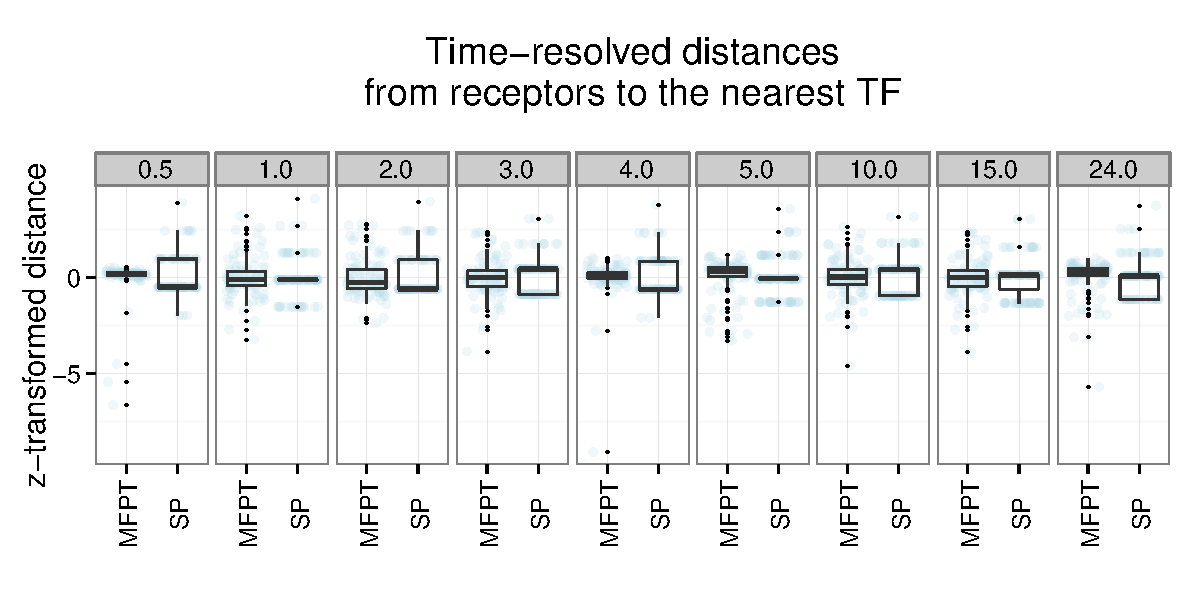
\includegraphics[width=\textwidth]{h838-mfpt_sp_z.pdf}
\end{center}
\caption[MFPT and SP distribution]{
{\bf Time-resolved distribution of MFPT and SP for receptors to the 
nearest transcription factor.} 
Shown are the boxplot of the standardized MFPT and SP distributions at 
different time points. Individual data points are blue-shaded, jittered
and superimposed on the boxplot.
}
\label{fig:h838_mfpt_sp}
\end{figure}

A hallmark of the eukaryotic genome is that individual genes are often 
regulated by multiple transcription factors that combinatorially bind to 
promoters of genes~\citep{Harbison2004}. Therefore, the activation of multiple transcription
factors is vital to the regulatory machinery, which might also result
in the signal flow from different membrane receptors.
We selected all receptors with a significantly short MFPT distance (below the 5\% 
quantile) to the transcription factor, and divided them into 5 different
functional groups (\ref{fig:h838_mfpt_ts}), which all have distinct
dynamics. Interleukin receptors in H838 cells are close to the transcription
factors at an early stage, likely 
transmitting the external stimulus signal from 0.5 to 10 hours after
the scratch. C-X-C chemokine receptors and TGF-$\beta$ family receptors
are likely responsible for the signal flow until 15h after scratch,
whereas interferon receptors and TNF family receptors have short distances
to the downstream transcription factors over the whole time span.
We also fitted the raw data points with a local polynomial regression
curve. It stands out that TNF family receptors both have a rich number
of close-to-TF receptors over time, and have a narrow confidence region
resulting from the fitting, which implies their robust role in the 
cellular signal flow. Moreover, the closeness between TNF family receptors
and TFs seems to be most prominent between 5 and 10 hours after the scratch.

\begin{figure}[!ht]
\begin{center}
\includegraphics[width=\textwidth]{h838-mfpt_ts.pdf}
\end{center}
\caption[Time course of the MFPT distance]{
{\bf Time course of the MFPT distance between the 5\% closest receptors
to transcription factors.} 
We plot the individual receptors (dots) and a LOESS (locally weighted 
scatterplot smoothing) regression curve to monitor the receptor dynamics,
the gray area is the 95\% confidence interval of the fit.
}
\label{fig:h838_mfpt_ts}
\end{figure}

As a more parsimonious ansatz, we also only look at the receptors with the 
minimal MFPT distance for each time point (\ref{fig:h838_mfpt_top}).
Under the assumption that only one receptor is responsible for the 
signal transduction at one time point, the picture becomes even clearer.
The interleukin and interferon receptors have the closest distances to
TFs at the beginning and end of the experiment respectively. TGF-$\beta$
and TNF family receptors drive the signal flow in turn, with TNF family
receptors having a more pronounced time window between 2 and 5 hours
after the scratch.

\begin{figure}[!ht]
\begin{center}
\includegraphics[width=\textwidth]{h838-mfpt_top.pdf}
\end{center}
\caption[Receptors with the shortest MFPT at each time point]{
{\bf The top-ranked receptors in terms of MFPT to TFs at each time point.} 
We show the top receptors with the shortest MFPT to TFs at each time point,
they consist of 4 groups, i.e. TNF family, TGF-$\beta$ family, interleukin and
interferon receptors.
}
\label{fig:h838_mfpt_top}
\end{figure}

%As depicted in \ref{fig:h838_receptor_ts_ex}, the inverse
%mean first passage time (MFPT) and inverse shortest path 
%(SP) show totally different dynamics. We further use the
%area under the curve (AUC) of inverse distances as a 
%measure of proximity and thus functional relatedness between
%receptors and transcription factors (TF). 
%The larger the AUC is,
%the more likely, we hypothesize, that the signal is
%transmitted through this receptor downward to the 
%corresponding TFs. We also calculate the probability of
%obtaining a certain AUC by chance, which is the fraction
%of AUC between the receptor and bootstrapped TFs that are
%more extreme than the actual AUC 
%(\ref{fig:h838_receptor_pval_ex}).
%
%\begin{figure}[!ht]
%\begin{center}
%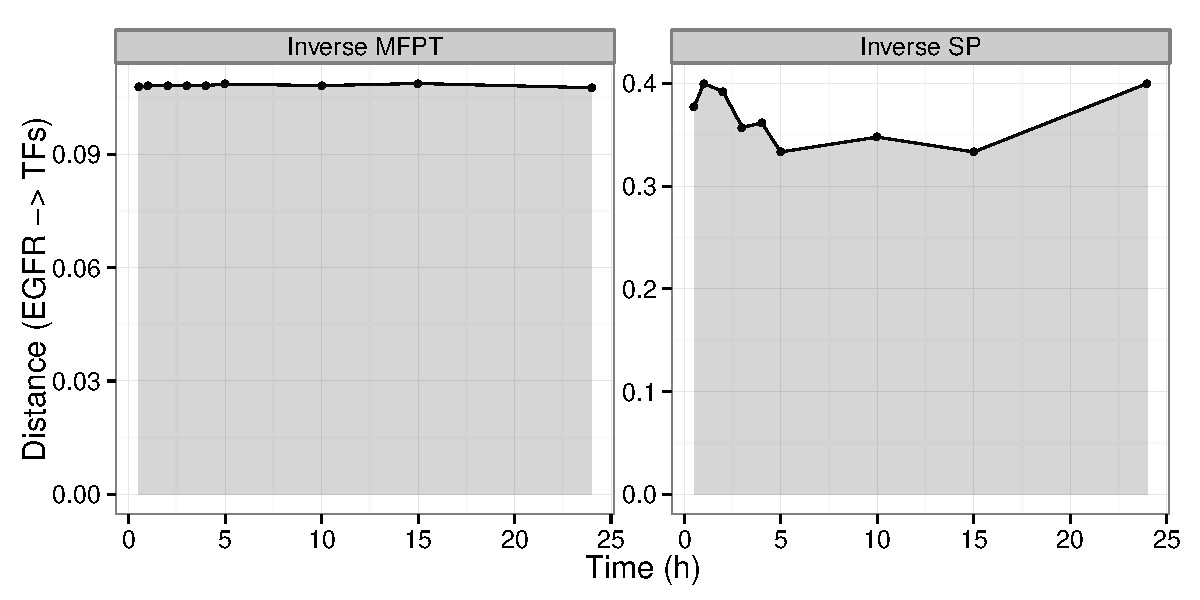
\includegraphics[width=\textwidth]{h838-receptor_ts_ex_hppi.pdf}
%\end{center}
%\caption[Inverse distance over time]{
%{\bf Inverse nodal distance from EGFR to enriched 
%transcription factors at each time point.} 
%Inverse distance is measured by mean first passage time
%(MFPT) and shortest path (SP) respectively. Shaded area
%indicates the area under the curve (AUC) used to 
%characterize the overall proximity between a given
%receptor and all enriched transcription factors.
%}
%\label{fig:h838_receptor_ts_ex}
%\end{figure}
%
%\begin{figure}[!ht]
%\begin{center}
%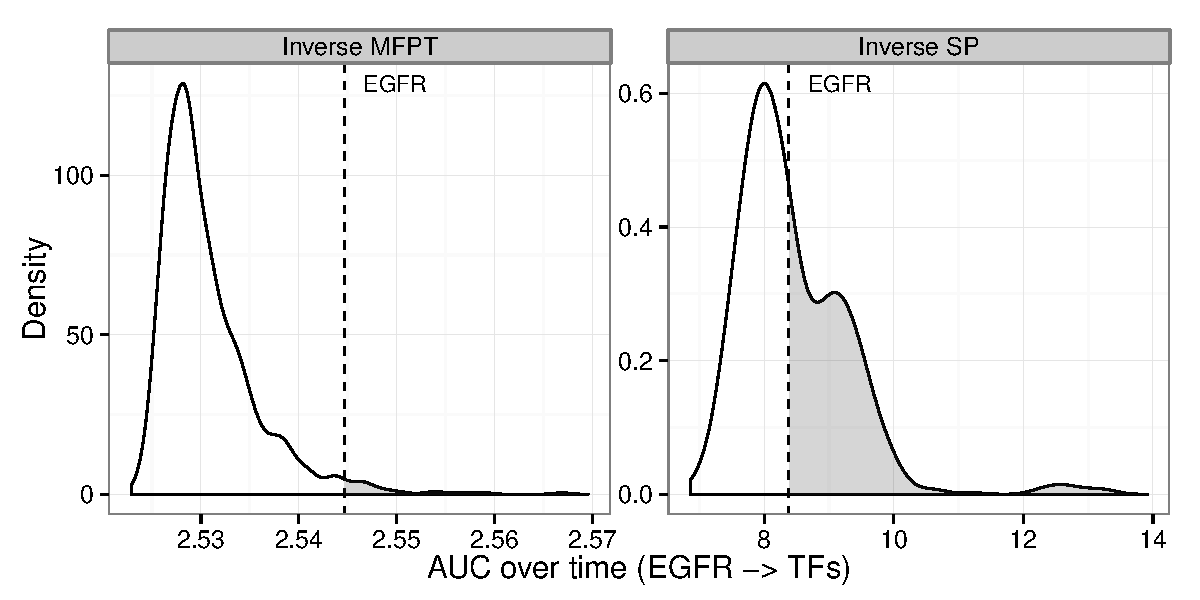
\includegraphics[width=\textwidth]{h838-receptor_pval_ex_hppi.pdf}
%\end{center}
%\caption[Significance of the inverse distance AUC]{
%{\bf Significance of the inverse distance AUC from EGFR to
%all enriched transcription factors.} 
%Shown is the distribution of the inverse distance AUC from
%EGFR to all enriched transcription factors (TF). 
%The distribution
%is determined by calculating the inverse distance between
%EGFR and randomly selected TFs.
%AUC is calculated for inverse MFPT and SP as in 
%\ref{fig:h838_receptor_ts_ex}. Dashed vertical line
%denotes the AUC from EGFR to the TFs identified from the
%data, shaded area is the region that the bootstrapped 
%AUC is more extreme than the actual value and is thus used
%to calculate the $p$-value.
%}
%\label{fig:h838_receptor_pval_ex}
%\end{figure}
%
%In summary, if we rank the receptors by their inverse
%shortest path AUC (\ref{fig:h838_receptor_auc_sp}), we
%can easily identify certain candidate receptors that
%are likely responsible for the signal flow from the external
%stimulus to the downstream transcription factors. 
%Interleukin and TNF receptors are two big families of 
%membrane receptors. Most of the interleukin receptors have
%a significant AUC as measured by the inverse shortest path,
%whereas none of the TNF receptor super family members has
%a $p$-value less than 0.05. Therefore, neither of both 
%classes provides a highly discriminative candidate receptor.
%Among the chemokine (C-X-C motif) receptors, CXCR4 stands
%out. In terms of the chemokine (C-C motif) receptors, 
%CCR5/1/2 are the hits that are most likely related to the
%signal flow. Yet other receptors can be identified that
%have both a high AUC and a significant $p$-value.
%In contrast, all receptors show a homogeneous distribution
%of both AUC and $p$-value when ranked according to the 
%inverse mean first passage time 
%(\ref{fig:h838_receptor_auc_mfpt}), which is thus of
%limited use in this specific case.
%
%\begin{figure}[!ht]
%\begin{center}
%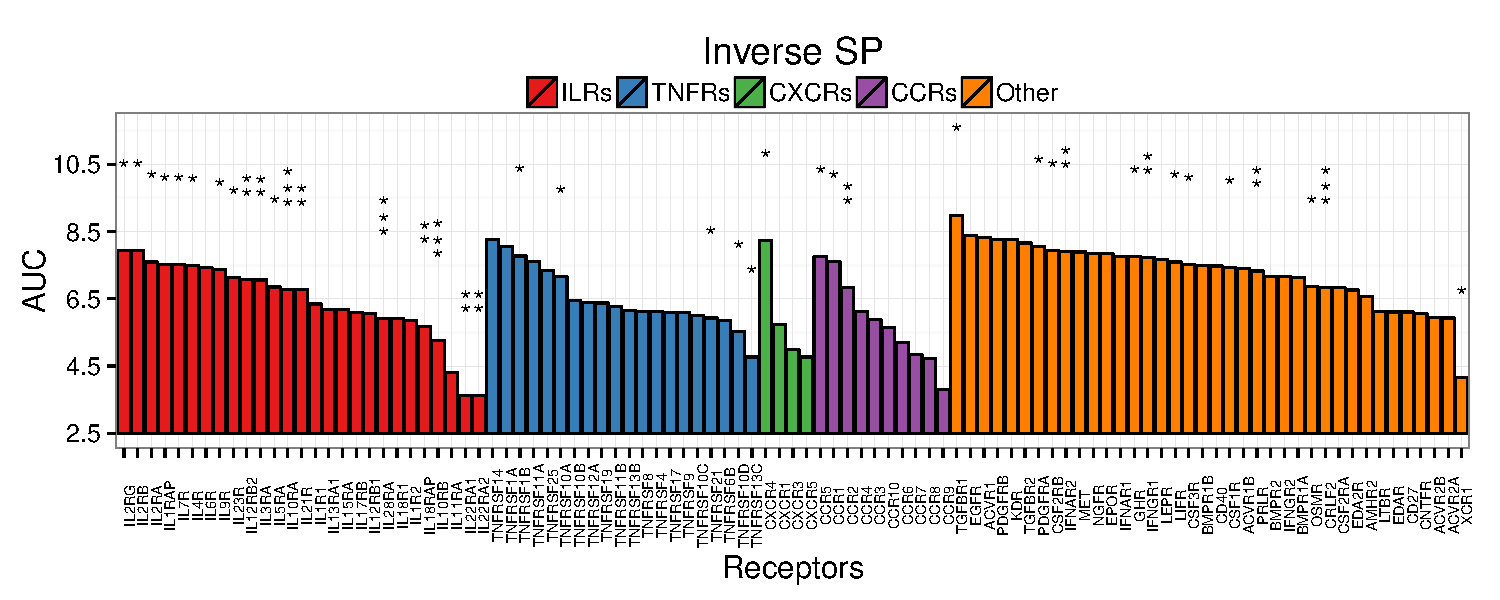
\includegraphics[width=\textwidth]{h838-receptor_auc_sp_hppi.pdf}
%\end{center}
%\caption[Receptor ranking by inverse SP]{
%{\bf Receptor ranking by the AUC of inverse shortest path.} 
%Receptors are grouped into 5 major categories and ranked
%according to their AUC of shortest path to all enriched TFs.
%Asterisks indicate the $p$-value of the AUC as determined by
%bootstrapping. ***: $p<0.01$, **: $p<0.05$, *: $p<0.1$.
%}
%\label{fig:h838_receptor_auc_sp}
%\end{figure}
%
%\begin{figure}[!ht]
%\begin{center}
%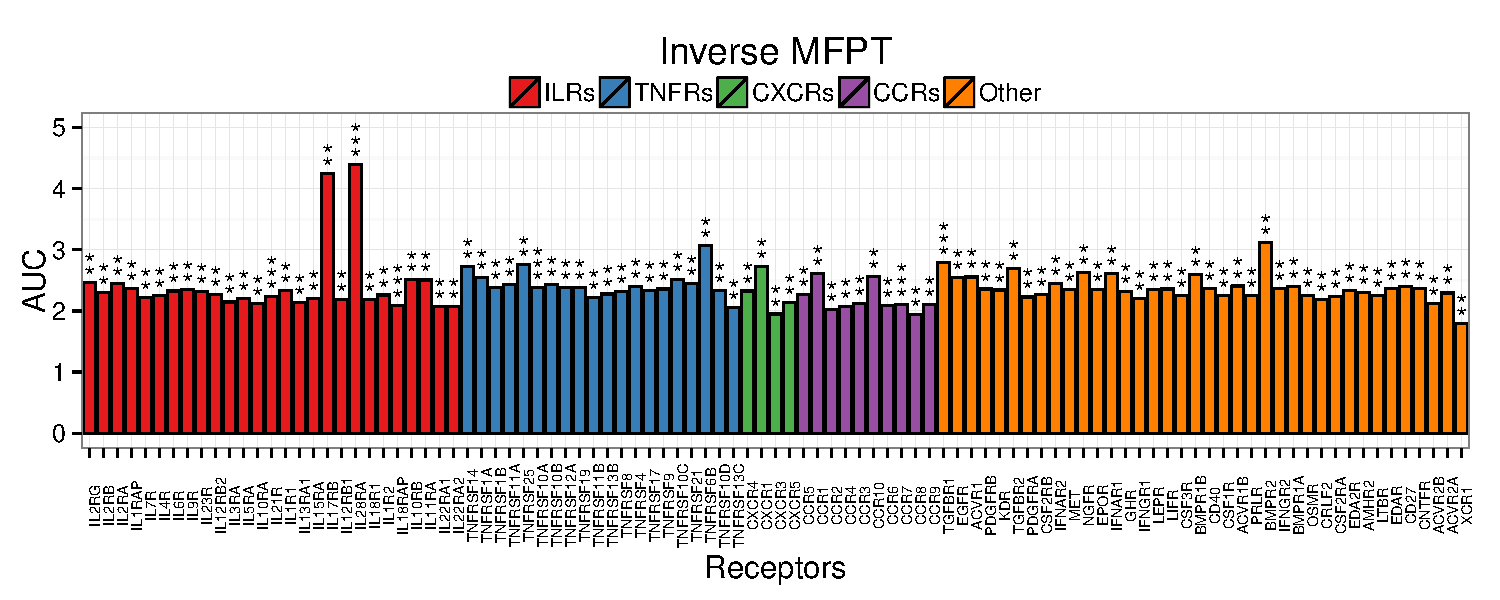
\includegraphics[width=\textwidth]{h838-receptor_auc_mfpt_hppi.pdf}
%\end{center}
%\caption[Receptor ranking by inverse MFPT]{
%{\bf Receptor ranking by the AUC of inverse mean first 
%passage time.} 
%Receptors are grouped into 5 major categories and ranked
%according to their AUC of MFPT to all enriched TFs.
%Asterisks indicate the $p$-value of the AUC as determined by
%bootstrapping. ***: $p<0.01$, **: $p<0.05$, *: $p<0.1$.
%}
%\label{fig:h838_receptor_auc_mfpt}
%\end{figure}
%
%\begin{figure}[!ht]
%\begin{center}
%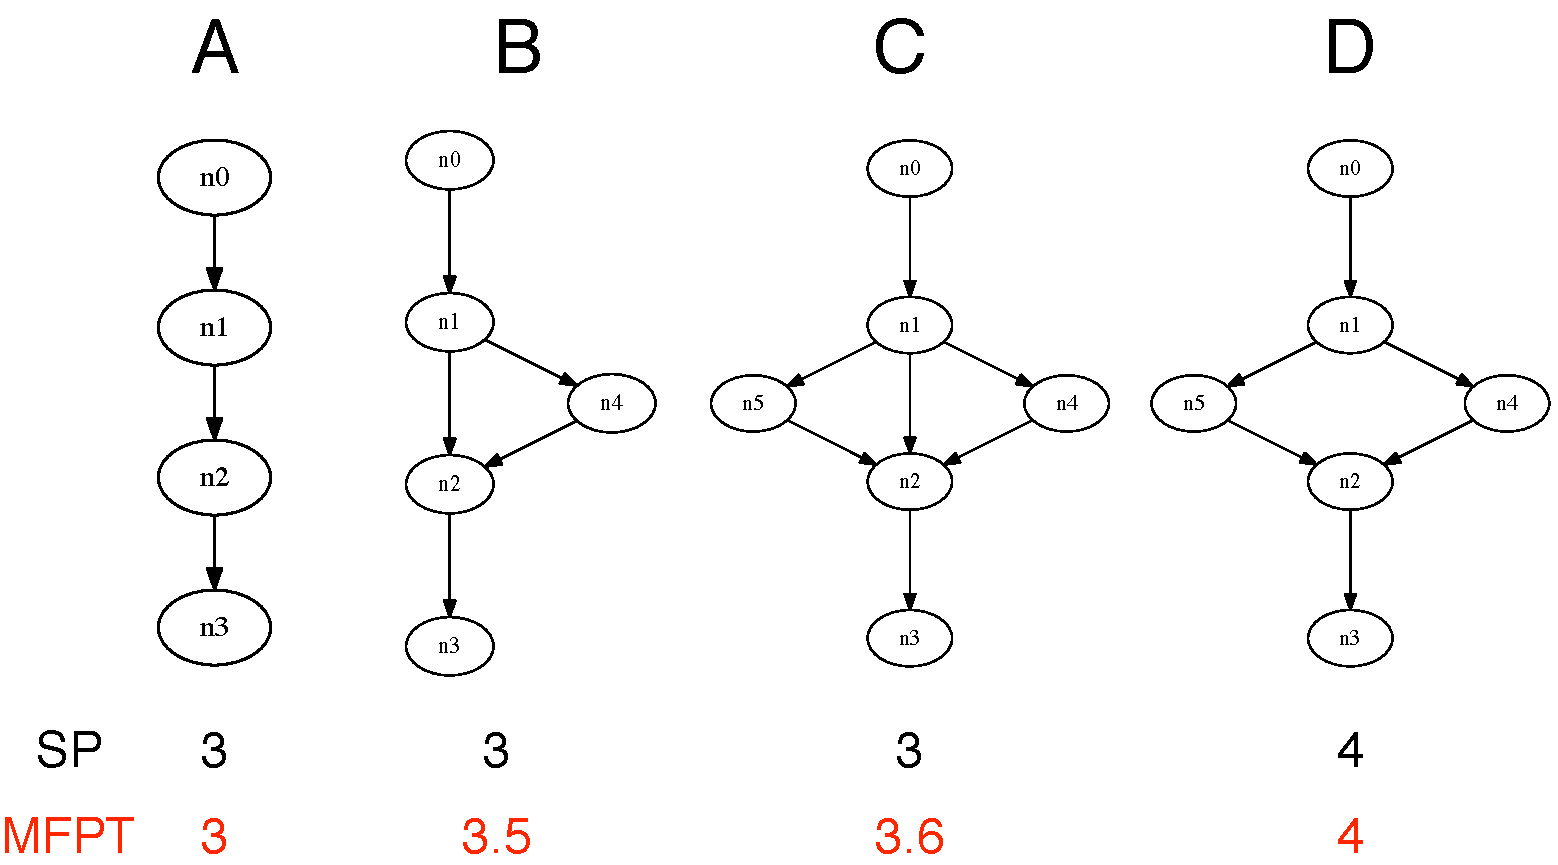
\includegraphics[width=\textwidth]{mfpt_directed_toy.pdf}
%\end{center}
%\caption[Toy example of SP and MFPT on different directed networks]{
%{\bf Comparison of shortest path (SP) length and mean first passage time 
%(MFPT) on different directed toy networks.}
%Shown are the distances between node $n0$ and $n3$ measured in shortest path 
%(SP) and mean first passage time (MFPT) respectively.
%}
%\label{fig:mfpt_directed_toy}
%\end{figure}

\subsubsection{Supernatant  from different co-cultures show distinct cytokine composition}

If the receptors predicted in the previous section are indeed of functional
relevance in the signal processing of tumor cells, we would also expect an
enrichment of the corresponding ligands in the medium,
which mediate the communication between
HPAEC and H838 cells and enhance the tumor cell migration.
To this end, we quantified the cytokine composition
of the  homo- and heterogeneous cocultures
both before and 24h after onset of migration.
We used a  fluorescent bead array based cytokine assay which detects fifty cytokines (\ref{table:cytokine}).
The quantification of fifty different analytes was performed and evaluated in a  fully automated 96-well format Luminex analysis system (Multimetrix, Regensburg,  Germany). 

\begin{longtable}{ccccc}
\caption{List of cytokines in the array.} \\ 
\hline
Eotaxin & IL-5 &   IP-10 &  HGF & MCP-3\\
\rowcolor{Gray} FGF basic &  IL-6 &   MCP-1 &  ICAM-1 & M-CSF\\
G-CSF &  IL-7 &   MIP-1$\alpha$ & IFN$\alpha$2 & MIF\\
\rowcolor{Gray} GM-CSF & IL-8 &   MIP-1$\beta$ &  IL-1$\alpha$ & MIG\\
IFN-$\gamma$ &  IL-9&    PDGF bb&  IL-11-R$\alpha$-lokus chemokine & SCF\\
\rowcolor{Gray} IL-1b &  IL-10 &  RANTES & IL-12 (p40) & SCGF-$\beta$\\
IL-1R$\alpha$ &  IL-12 (p70) &  TNF$\alpha$ &   IL-16 &  SDF-1$\alpha$\\
\rowcolor{Gray} IL-2 &   IL-13 &  VEGF &   IL-18 &  TNF$\beta$\\
IL-3 &   IL-15 &  $\beta$-NGF&  IL-2R-$\alpha$ &   TRAIL\\
\rowcolor{Gray} IL-4 &   IL-17 &  GRO$\alpha$ &  LIF &VCAM-1\\
\hline
\label{table:cytokine}
\end{longtable}
\newpage

A total of twenty-four different cytokines were present in detectable amounts,
fifteen of which showed significant differential upregulation
(\ref{fig:cytokine} A).
% Should add here an additional table with the quantification of all cytokines
Gro-$\alpha$, MCP-3, IL-6, IL-8, IL-13, FGF basic, G-CSF, IP-10 and RANTES were
upregulated in the heterogeneous coculture prior to cell migration.
MIF, IL-12, IL-15, MCP-1 and TNF-$\alpha$ were also upregulated
in the heterogeneous cocultures, and this upregulation was increasing
during tumor cell migration.
Finally, SDF-1$\alpha$ was only found in the heterogeneous coculture,
and was also upregulated after scratching. 

% Need a better headline for the subsection here 
\subsubsection{Isolation of cytokines relevant to migration}

Based on the cytokine array results and the receptor inference from random walk, 
we found that 
%the upregulated \sdfonea,
%RANTES, MCP-1 are the ligands for CXCR4, CCR5/1/2 respectively and thus agrees
%with the shortest path prediction very well. 
\tnfa, \sdfonea and several interleukins have both enriched ligands in the medium and
the corresponding receptors that are close to the downstream enriched 
transcription factors.
%representative cytokines from the interleukin and TNF
%family, which are also known to play a role
%in cell migration in general.
% need some idea why we did not add MIF to the candidate list
%(TNF-$\alpha$, IL-6, RANTES, SDF-1$\alpha$, MCP-1, IL-8, Gro-$\alpha$).

To test the influence of the above factors on tumor cell migration,
we analysed scratch assays of H838 monocultures under the influence of 
individual or multiple of these cytokines. 
Furthermore, we added VEGF to the candidate list for its known involvement in
angiogenesis and metastasis of tumor cells~\citep{Ferrara2003,Hiratsuka2002} and GRO-$\alpha$ as a ligand for CXCR2, which is also highly expressed in the medium.
Comparing migration areas after 24h, 
we found that only IL-6, TNF-$\alpha$ and SDF-1$\alpha$ significantly 
increase the migration of H838 cells (\ref{fig:cytokine} B, two-sided $t$-test,
$p < 0.05$). 
To further corroborate this result, we neutralized 
TNF-$\alpha$ and SDF-1$\alpha$ in heterogeneous cocultures  by adding neutralizing antibodies.
Inhibition of  either TNF-$\alpha$ or SDF-1$\alpha$ significantly reduced tumor cell migration (\ref{fig:cytokine} C). 
Simultaneous inhibition of TNF-$\alpha$ and SDF-1$\alpha$ did not result in an additive effect, yet increased the statistical significance of the migration 
inhibition
(two-sided $t$-test, $p=1.6\times10^{-4}$).

\begin{figure}
\begin{center}
%\captionsetup{labelformat=prepage}
%\newpage
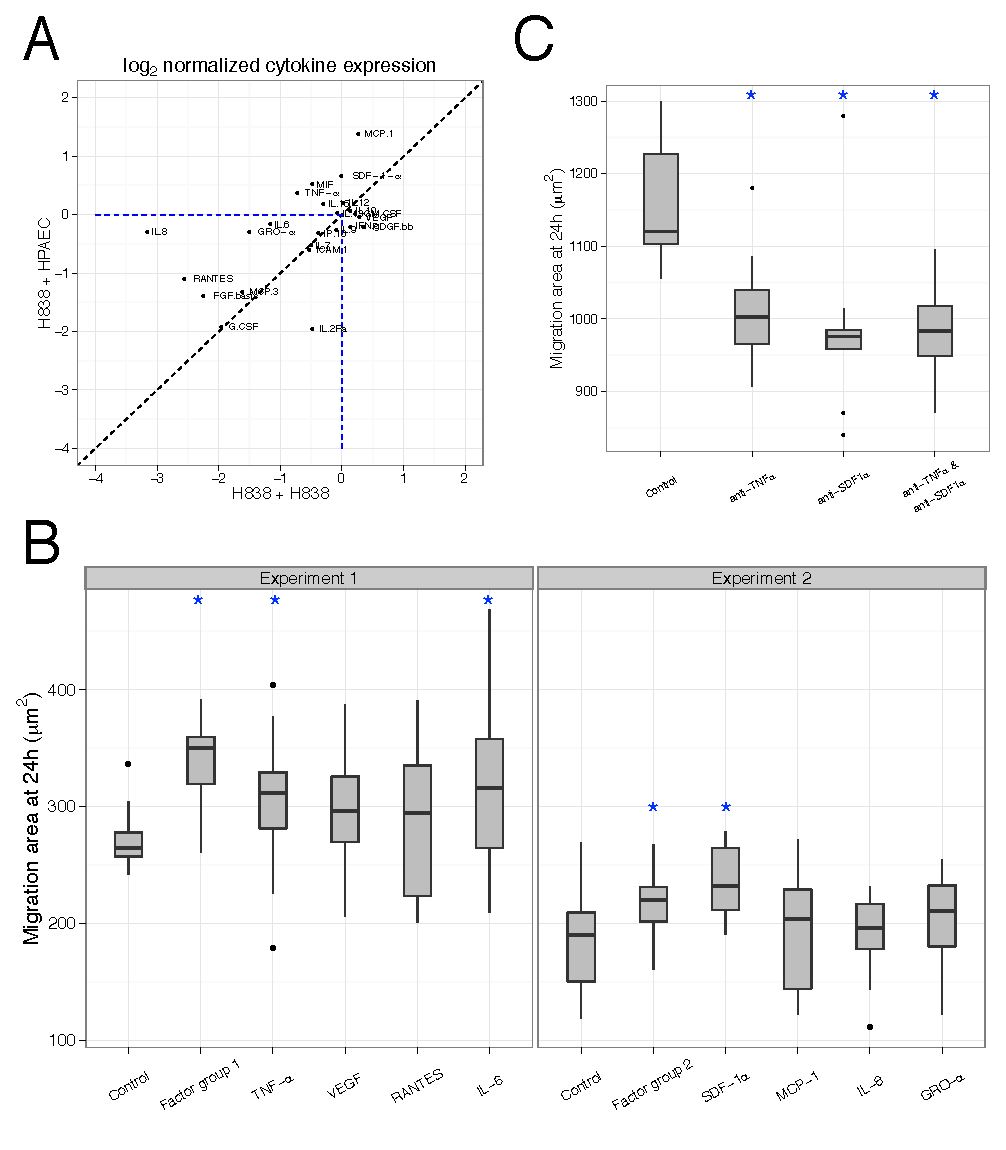
\includegraphics[width=\textwidth]{fig-cytokine.pdf}
\end{center}
\caption[Verification of key cytokines]{
{\bf Verification of key cytokines involved in the tumor cell migration.} 
(A) $\log_2$ transformed ratios of cytokine expression in heterogeneous respective
homogeneous coculture are shown. The black dashed line with a slope of 1 denotes 
the identity and the blue dashed lines denote the zero $\log_2$ fold change
or equal amount of cytokines between the scratched and unscratched conditioned 
media.
(B) Migration area of H838 cells at 24h after scratch in the H838 mono-culture 
treated with the 8
factors, the 2 factor groups and as in the control experiment.
(C) Migration area of H838 cells at 24h after scratch in the heterogeneous 
H838/HPAEC coculture 
treated with the neutralizing antibodies against TNF-$\alpha$, SDF-1$\alpha$
and both together. Asterisks in all plots denote that data are significantly 
different from the control according to a two-sided $t$-test ($p < 0.05$).
}
\label{fig:cytokine}
%\end{center}
\end{figure}

\subsubsection{Cytokine genes are expressed differently in H838 and HPAEC}

To elucidate the origin of the cytokines that have an impact on the tumor
cell migration,
we investigated the gene expression profiles of
our previously identified cytokines of interest in both H838 and HPAEC cells. 
%We compared the basal 
%expression levels of all genes with protein products
%annotated as cytokines in the KEGG cytokine-cytokine receptor interaction pathway. 
%However, none of the cytokine encoding genes 
%showed a differential basal regulation between the two coculture conditions. Over time, IL6 and CXCL14 are significantly
%down-regulated, and CSF1 is significantly up-regulated. 
Neither \tnfa nor \sdfonea in the H838 cells
responds differentially during H838 migration (\ref{fig:cytokine_dynamic} A).
However, 
an RT-qPCR experiment confirmed an early and transient response of  
TNF-$\alpha$ as well as a later and prolonged upregulation of 
SDF-1$\alpha$ in the HPAEC cells (\ref{fig:cytokine_dynamic} B). 
% maybe put this figure into the supplement
%Looking at the basal expression levels within each culture condition, only five out of 162 cytokines (IL18, IL10, PDGFC, BMP7 and TNFSF12) 
%had a significantly high expression level in both conditions
%(\ref{fig:cytokine_basal}), 
%and none of these could be directly related to the migration-enhancing 
%cell-cell communication.

%\begin{figure}[!ht]
\begin{center}
\captionsetup{labelformat=prepage}
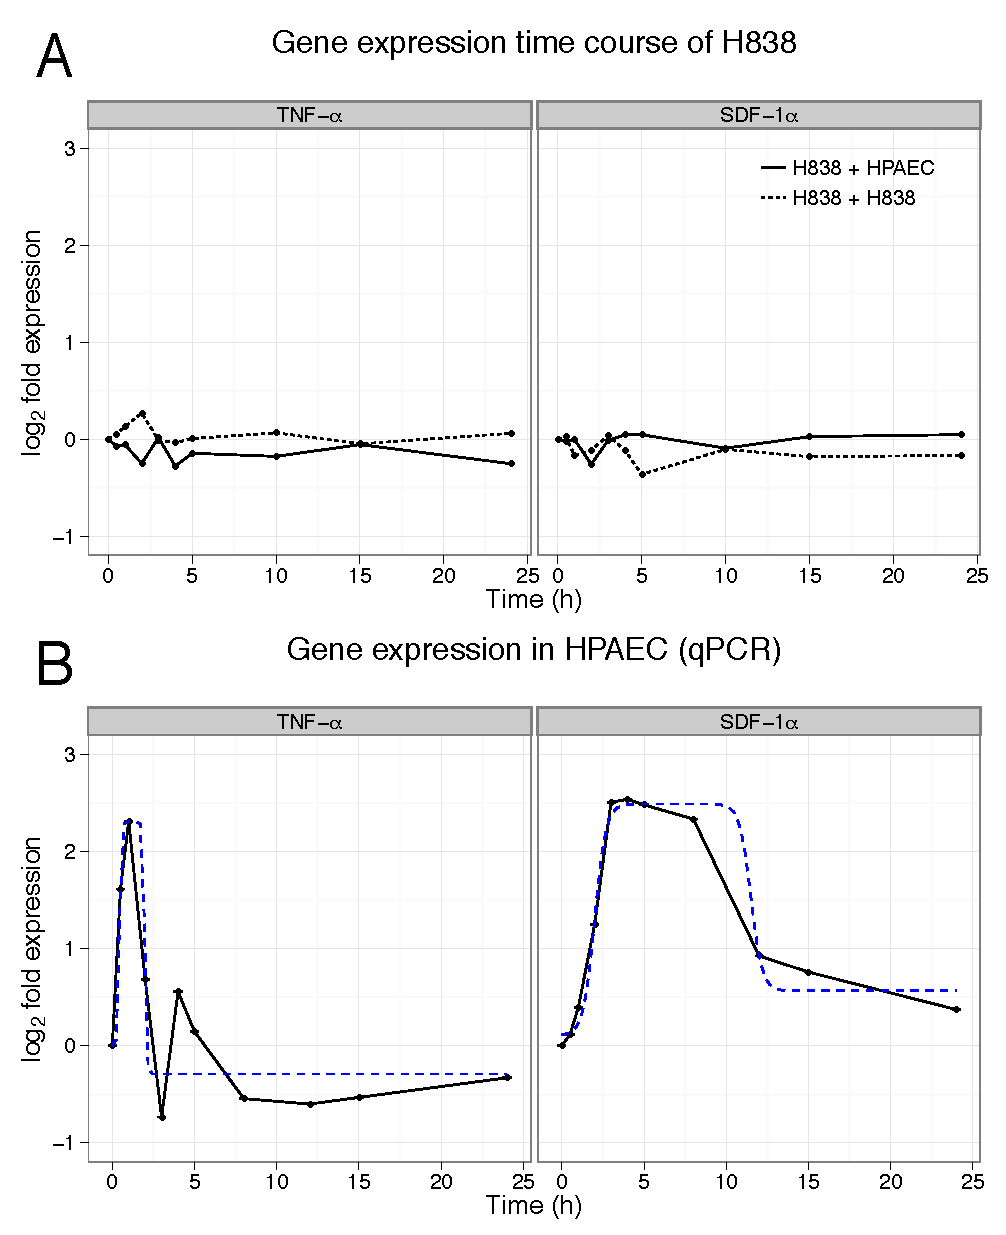
\includegraphics[width=\textwidth]{fig-cytokine_dynamic.pdf}
\newpage
%\end{center}
\captionof{figure}[Gene expression of \tnfa and \sdfonea]{
{\bf mRNA of TNF-$\alpha$ and SDF-1$\alpha$ is regulated in HPAEC instead of H838 
cells.}
(A) $\log_2$ fold expression of TNF-$\alpha$ and SDF-1$\alpha$ (CXCL12) in H838 
cells plotted
over time for the hetero- and homogeneous coculture respectively.
(B) $\log_2$ fold expression of TNF-$\alpha$ and SDF-1$\alpha$ in HPAEC cells 
from the qPCR
experiment in the heterogeneous coculture plotted
over time. Blue dashed lines denote the impulse model fit~\cite{Chechik2009}.
}
\label{fig:cytokine_dynamic}
%\end{figure}
\end{center}

%\begin{figure}[!ht]
%\begin{center}
%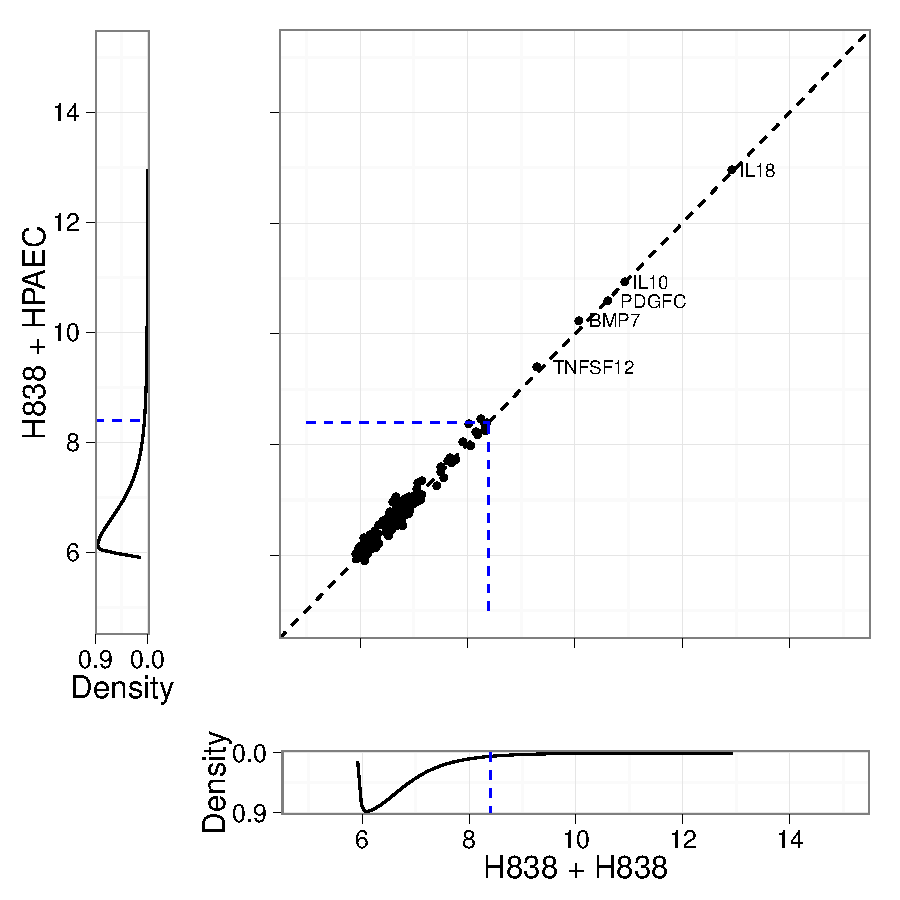
\includegraphics[width=\textwidth]{fig-basal_cytokine.pdf}
%\end{center}
%\caption[Basal cytokine gene expression]{
%{\bf Few cytokines highly expressed in H838 at 0h.}
%Comparison of $\log_2$ transformed basal mRNA intensities at 0h of all 
%cytokines annotated 
%in the KEGG \emph{cytokine-cytokine receptor interaction pathway} between
%the hetero- and homogeneous coculture. Blue dashed lines denote the significance
%level ($p=0.05$) after fitting the basal expression distribution with a skew-$t$ 
%distribution~\cite{Azzalini2003}. Only IL18, IL10, PDGFC,
%BMP7 and TNFSF12 are above this threshold in both conditions, 
%i.e. significantly up-regulated
%at 0h.
%}
%\label{fig:cytokine_basal}
%\end{figure}

We conclude that the cytokines in the supernatant that can drive the migration
phenotype
must originate primarily from the HPAEC cells.  
\sdfonea is expressed in the HPAEC cells with both a delay and a longer peak duration.
By fitting the qPCR time course with an impulse model 
(\ref{sec:impulse}), which measures the peak 
duration as the 
temporal difference between the inflection points of two
sigmoidal curves, 
% add this in materials and methods
we obtain an activation duration of  8.3 hours and 1.6 hours for SDF-1$\alpha$
and TNF-$\alpha$, respectively.

\subsection{Discussion}

The key medical problem in lung cancer and its predominant type non-small 
cell lung carcinoma (NSCLC) is an early systemic metastatic spread of tumor cells 
independent of tumor size, which leads to high mortality rate. Tumor progression 
and metastasis is regulated by many different processes, inter alia by interactions 
via soluble factors between tumor cells and cells of tumor microenvironment, such as 
endothelial cells. In this study, we analyzed the interactions between NSCLC cells 
and endothelial cells and their influence on NSCLC cell migration. We identified 
two key cytokines, TNF-$\alpha$ and SDF-1$\alpha$, that are expressed by the 
endothelial cells and promote the migration of NSCLC cells.

In this study, we verified that TNF-$\alpha$ and SDF-1$\alpha$ are two
key cytokines that are expressed by the endothelial cells and promote the migration
of tumor cells. We proposed a two-step approach to link the transcriptome response
with the causal signal flow in the protein interaction network. First, gene set
enrichment analysis was applied to infer the sequence of transcription factor
activation that results in the gene expression. Second, we predicted several
putative receptors that are most closely linked to the downstream transcription
factors based on 
a random walk approach in the interactome. Among all candidate receptors,
TNF-$\alpha$ and SDF-1$\alpha$ receptors have a direct effect on the phenotype,
and the inhibition of the respective ligands leads to reduced migration 
activity. We further
hint at endothelial cells as possible sources for \tnfa and \sdfonea.

We discuss next about endothelial cell-tumor cell communication, what is known and what we found at the transcription and protein level.
We also speculate the role of \tnfa and \sdfonea in tumors and especially lung tumors.

\begin{itemize}
\item \textbf{What do we know about \tnfa and \sdfonea with respect to tumor cell migration?}

\tnfa was first identified as an anti-tumor cytokine that is involved in the killing
of certain kinds of tumors, however, it is appreciated recently that \tnfa can also 
act as a tumor-promoting factor and enhance tumor growth and metastasis%
~\citep{Wu2010}. It has also been shown in the ovarian cancer cells cocultured with
macrophages that \tnfa can induce the up-regulation of 
CXCR4 mRNA, which is the receptor of \sdfonea. This response to \tnfa involves both
AP-1 and NF-$\kappa$B related pathways~\citep{Kulbe2005}. Blocking the \tnfa receptor
in mouse Lewis lung carcinoma cell cultures decreases the gene expression of CXCR4~%
\citep{Sasi2011}.

It has been shown that the \sdfonea/CXCR4 pathway has pleiotropic activities and it 
promotes tumor growth and malignancy, enhances tumor angiogenesis, participates in tumor metastasis, and contributes to immunosuppressive networks within the tumor microenvironment~\citep{Kryczek2007}. 
Recently, it has also been shown that a special NSCLC cell line expresses a
high amount of CXCR4 and has cancer stem-like cell functions. The CXCR4-mediated
signaling is likely relayed by STAT3~\citep{Jung2013}.
Both stroma and cancer cells can produce \sdfonea, 
although in our system it is mainly expressed by the endothelial cells. In the presence of neutralizing \sdfonea antibodies, NSCLC tumor metastases were also significantly reduced~\citep{Phillips2003}.

The identification of \tnfa as a key stroma-originating factor that promotes 
tumor cell migration is of great interest, since its release is a general response to chemotherapy in different stromal cell types~\citep{Acharyya2012}. Together with
other cytokines, such as HGF, that contribute to the drug resistance of cancer
treatment~\citep{Straussman2012}, these soluble factors in the tumor microenvironment
might be the key to the adverse effects in the cancer therapy and the potential target of intervention.


\item \textbf{What is new in our methods?}

The advantage of our two-step integrative approach to identifying 
relevant transcription factors that lead to the transcriptome response
and the signal flow in the protein interaction network 
is at least two-fold: first, we apply gene set enrichment test to avoid the hard 
significance cutoff in the conventional hypergeometric test and at the same time
to detect weak but coordinated regulation of transcription factor targets. This is 
necessary since the tumor cell transcriptome does not show significantly
differential regulation between the homo- and heterogeneous coculture 
(\ref{fig:h838_transcriptome}) although they differ in the phenotype, which 
hints at a lack of correlation between the mRNA expression level and the protein 
activity. This in turn underlines the rationale behind the time-scale separation
in our approach. 

Second, due to the decoupling between the mRNA and protein
activities, it is vital to consider signaling pathways not directly represented
in the transcriptome data, but rather embedded in the protein interaction network
instead. In order to infer the signal flow from the membrane receptors to 
transcription factors, we simply assume that the signal traverses the most efficient
path connecting a certain pair of receptor and transcription factor, which is 
defined by the mean first passage time of a random walker and takes into account
the global topology of the protein interaction network.

\item \textbf{What new  biological insights do we gain?}

The combination of the random walk approach, cytokine array and single factor
stimulation together confirms the involvement of \tnfa and interleukins in the
signal flow and phenotype development of the tumor cells. The fact that \sdfonea
is only present in the tumor-endothelial cell heterogeneous coculture makes it
also a candidate in the migration determination, which is also validated by the 
single factor stimulation and neutralizing antibody experiments.

Based on our time-resolved qPCR results, we conclude that \tnfa in the endothelial 
cells is 
transiently expressed and peaks earlier than \sdfonea, which is in line with
the random walk prediction that TNF familiy receptors are strongly linked to
the transcription factors between 2 and 5 hours after the scratch. This receptor
wave in the H838 cells lags behind the ligand transcript level in the HPAEC cells,
and is also more sustained, possibly due to certain positive feedback mechanisms.
\sdfonea, in contrast, has
a longer activation time window. These results are in line with the hypothesis 
that \tnfa induces the CXCR4 expression in tumor cells, which can then respond
to \sdfonea. Nevertheless, CXCR4 in the lung cancer cell line H838 is neither
basal highly expressed (Benjamini-Hochberg corrected $p$-value = 0.7977245), nor differentially regulated over time (Benjamini-Hochberg
corrected $p$-value = 0.893767) in the 
heterogeneous coculture of tumor and endothelial cells, which indicates that
cytokine receptors important for the communication with endothelial cells might
only be regulated at the protein level.

According to the transcription factor target enrichment analysis, target genes
of AP-1 are more significantly upregulated within the first two hours. 
%whereas those
%of NF-$\kappa$B are only activated between 12 and 16 hours, although both AP-1 and
%NF-$\kappa$B are known to be involved in the \tnfa induced response~%
%\citep{Kulbe2005}. 
Taking into account
the early expression peak of \tnfa in the endothelial cells, it seems
in our particular coculture system of H838 and HPAEC cells, the initial 
transcriptome response in the tumor cells might be mediated through the AP-1
related pathway~\citep{Kulbe2005}. It has also been
shown that the CXCL12/CXCR4 activation of NSCLC cell lines 
increased intracellular calcium mobilization and MAP kinase 
activation with enhanced ERK1/2 phosphorylation~%
\citep{Belperio2004}, which is 
known to be upstream of the AP-1 transcription complex.
Adding to the observation that the MAP kinase pathway genes are also enriched 
in the tumor cells of the heterogeneous coculture, 
all evidence points to the important role of the
AP-1 complex in the tumor cells to convey the information of  
the \sdfonea/CXCR4 activation from the microenvironment and to initiate cell
migration~\citep{Busch2008,Singh2012}.

Cell-cycle related transcription factors E2F has been linked with the chemokine
receptor CXCR4 in neurons. The transcriptional activity of E2F is either 
increased or decreased depending on the type of the CXCR4 ligand~\citep{Khan2003}.
The identification of E2F family proteins as activated transcription factors 
between 3 and 10 hours in the tumor cell also correlates with the expression of 
the CXCR4 ligand \sdfonea by endothelial cells within the same time frame.

\item \textbf{Limitations}

One of the fundamental assumptions about the interactome analysis that links receptos
and transcription factors is that the network is static. However, one can 
easily imagine that the protein interactions can be highly context/condition
dependent~\citep{Przytycka2010b,Schaefer2013}. This could be due to the wiring efficiency
and adaptability of the network under different stimuli, or it is simply 
a result of the biased data collection. Different experimental
techniques favor different types of interactions, e.g. yeast two-hybrid 
preferentially detects pairwise interactions and affinity purification
followed by mass spectrometry tends to find stable complexes of proteins.

The time-resolved transcriptome data provide a basis for deciphering the
sequential events at the transcriptional regulation level and also the 
different signal flow paths over time. In this work, however, we primarily
focus on the feedforward unidirectional flow from the receptor, through
transcription factors, to the target genes. There is a lack of the 
feedback mechanism which could occur either at the transcriptional
regulation level or directly at the receptor protein level. The sustained 
close link
between TNF family receptors and transcription factors from 2 to 5 hours
after the scratch could be the result of a positive feedback loop.

As with any other network analysis, our results highly depend on the quality of
the network data. More and more research has now addressed the assignment of
a confidence score to protein-protein interactions~\citep{Kamburov2012}.
Our choice of a confidence cutoff is essentially a trade-off between keeping
an intact network and ensuring a high data quality at the same time.

%By analyzing the shortest paths between receptors and transcription factors, 
%we classified \tnfa and \sdfonea related 
%pathways into the homogeneous and
%heterogeneous response pattern respectively. Taking into account the different
%expression dynamics of both cytokines in the endothelial cells, this implies a
%complementary role \tnfa and \sdfonea play in the enhancement of lung cancer
%cell migration. It could be that the transient expression of \tnfa by the 
%endothelial cells initiates a first but unspecific response in the tumor cells,
%while the secondary prolonged stimulation from \sdfonea leads to a signal that 
%propagates preferentially 
%on a more specific set of paths to the downstream transcription factors, which
%ultimately determines \emph{point of no return} of the enhanced migration phenotype 
%in the tumor cells.

%\begin{figure}[!ht]
%\hskip 0.5in A \hskip 2.5in B
%\begin{center}
%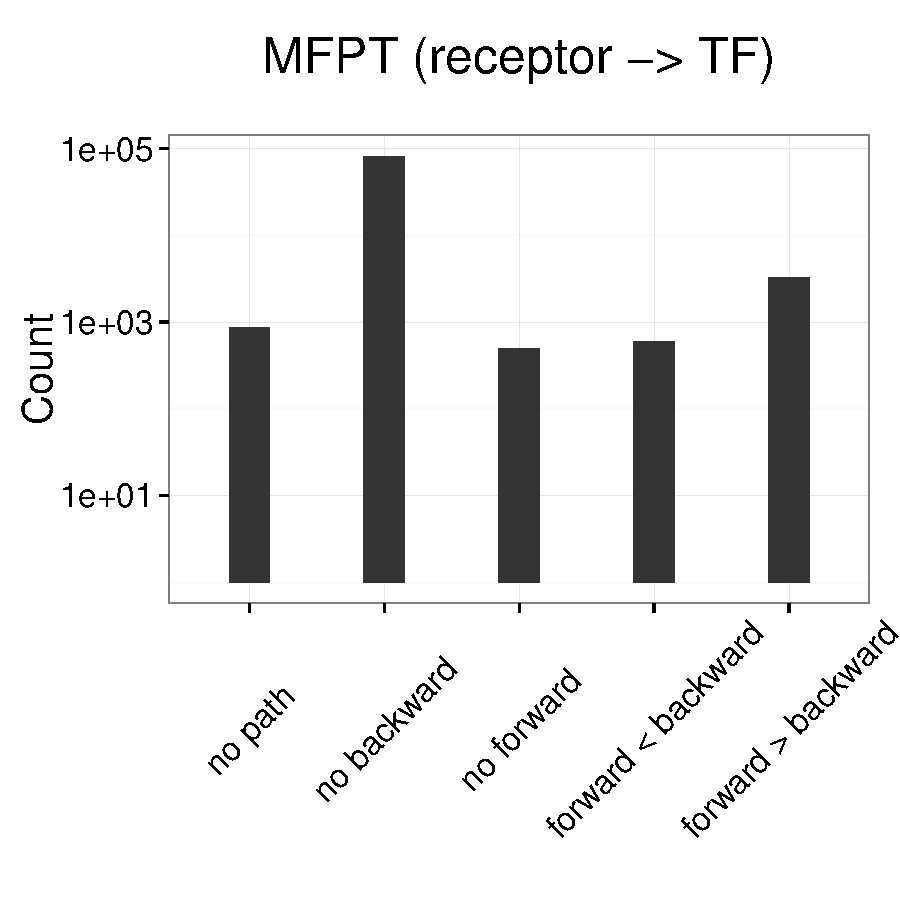
\includegraphics[width=0.45\textwidth]{mfpt-directed_bar.pdf}
%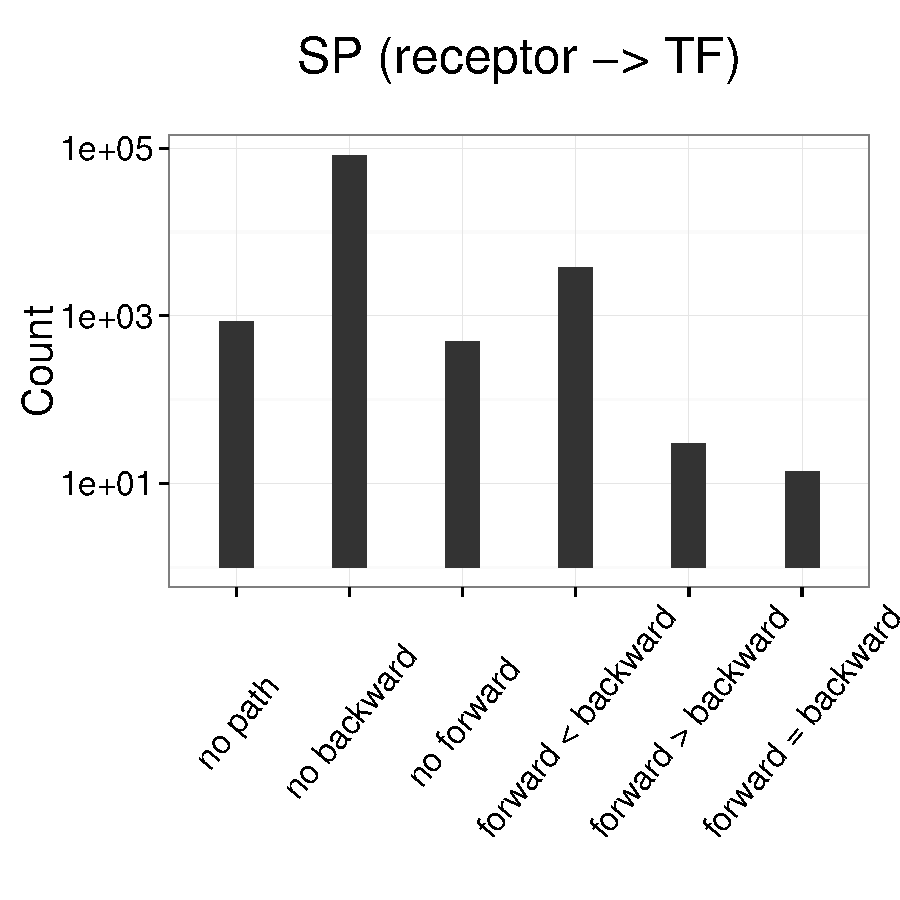
\includegraphics[width=0.45\textwidth]{sp-directed_bar.pdf}
%\end{center}
%\caption[Differential basal and dynamic gene expression]{
%{\bf Differential basal and dynamic gene expression in homo- and heterogeneous 
%cocultures.} 
%(A) Histogram of the differential gene expression at 0h as determined by limma~%
%\citep{Smyth2004}. 
%Basal differential expression is 
%represented as the negative log-transformed and multiple
%testing corrected $p$-value of the limma test.
%(B) Histogram of the differential gene expression over time as determined by the
%full/reduced model fitting~\citep{Mar2009}.
%Dynamical differential expression is 
%represented as the negative log-transformed and multiple
%testing corrected $p$-value of the full/reduced model
%likelihood ratio test.
%}
%\label{fig:mfpt_sp_bar}
%\end{figure}

\end{itemize}








